%\documentclass[useAMS,usenatbib]{mn2e}
%\bibliographystyle{mn2e}

\documentclass[a4paper,11pt]{article}
%\pdfoutput=1
%\pdfminorversion=5

\usepackage{jcappub}
%\usepackage{widetext}
\usepackage{graphicx}
%\usepackage{dcolumn}
\usepackage{bm}
\usepackage{amssymb,amsmath,bm,dsfont}
\usepackage{color}
\usepackage[dvipsnames]{xcolor}
%\usepackage[colorlinks,linkcolor=red,citecolor=blue,urlcolor=blue ]{hyperref}
%\usepackage{multirow}
\usepackage[utf8]{inputenc}
\usepackage{balance}
\usepackage{enumitem}
\usepackage{lipsum}
\newcommand{\nv}{\hat{\mathbf{\theta}}}
\newcommand{\kalo}{Karhunen-Lo\`{e}ve~}
\newcommand{\cfh}{CFHTLenS~}
\newcommand{\jcap}{JCAP}
\newcommand{\mnras}{MNRAS}
\newcommand{\aap}{A\&A}
\newcommand{\aaps}{A\&AS}
\newcommand{\apjs}{ApJS}
\newcommand{\apj}{ApJ}
\newcommand{\apjl}{ApJL}
\newcommand{\prd}{Phys.~Rev.~D}
\newcommand{\prl}{Phys.~Rev.~Lett.}
\newcommand{\aj}{Astron. Journal}
\newcommand{\pasp}{Publications of the ASP}
\newcommand{\nar}{New Astronomy Review}
\newcommand{\procspie}{Proceedings of the SPIE}
\newcommand{\physrep}{Physics Reports}

\newcommand{\todo}[1]{{\bf TODO: #1}}
%\newcommand{\todo}[1]{$\,$}

\newcommand{\PCL}{pseudo-$C_\ell$~}
\newcommand{\pcl}[3]{\hat C_{#1}^{#2 #3}}
\newcommand{\avg}[1]{\langle #1 \rangle}
\newcommand{\fsky}{f_{\mbox{\rm sky}}}
\newcommand{\clth}{C_\ell^{th}}
\newcommand{\clf}{C_\ell^{fore}}
\newcommand{\cl}{C_\ell}
\newcommand{\summ}[1]{\sum_{\bf #1}\Delta #1^2}
\newcommand{\Ylm}[3]{{\sf E}^{#1}_{\bf #2}({\bf #3})}
\newcommand{\red}[1]{{\color{red} #1}}

%\title[Disconnected pseudo-$C_\ell$ covariances for projected datasets]{Disconnected pseudo-$C_\ell$ covariances for projected datasets}
\title{Disconnected pseudo-$C_\ell$ covariances for projected datasets}

\author[a,b,1]{Carlos Garc\'{i}a-Garc\'{i}a}
\author[b,1]{David Alonso}
\author[b,1]{Emilio Bellini}

\affiliation[a]{Instituto de Física Fundamental, Consejo Superior de Investigaciones Científicas, c/. Serrano 123, E–28006, Madrid, Spain}
\affiliation[b]{Oxford Astrophysics, Department of Physics, Keble Road, Oxford, OX1 3RH, UK}

\emailAdd{carlosgarcia@iff.csic.es}
\emailAdd{david.alonso@physics.ox.ac.uk}
\emailAdd{emilio.bellini@physics.ox.ac.uk}

\abstract{\lipsum[1]}

\begin{document}
  \maketitle
  \flushbottom

\section{Introduction}
    
\section{Analytical Gaussian covariances}

  \subsection{Preliminaries}\label{ssec:theory.prelim}
    \todo{cites everywhere}
    We will deal with spin-0 and spin-2 fields defined on a 2-dimensional space. We will use a generic notation that can then be applied to both curved and flat skies. Given a field ${\bf a}({\bf x})$, with 1 (spin-0) or 2 components (spin-2), and defined on the coordinates ${\bf x}$, we define its generalized Fourier coefficients as
    \begin{equation}
      {\bf a}_{\bf k}=\summ{x}\,\Ylm{\dag}{k}{x}\,{\bf a}({\bf x}),
    \end{equation}
    where the operator $\summ{x}$ denotes a integral or sum of all coordinates ${\bf x}$, and $\Ylm{\dag}{k}{x}$ are a set of orthogonal functions. We will also assume that the $\Ylm{\dag}{k}{x}$ are a \emph{complete} set of basis functions, in which case:
    \begin{align}
      &\summ{x}\,\Ylm{\dag}{k}{x}\Ylm{}{l}{x}=\mathds{1}\Delta^x({\bf k},{\bf l}),\\
      &\summ{k}\,\Ylm{}{k}{x}\Ylm{\dag}{k}{y}=\mathds{1}\Delta^k({\bf x},{\bf y}),
    \end{align}
    where $\summ{k}$ denotes an integral over all possible generalised Fourier coefficients ${\bf k}$, and $\Delta^x$ and $\Delta^k$ are generalized delta functions:
    \begin{align}
      &\summ{k}\,f({\bf k})\Delta^x({\bf k},{\bf l})\equiv f({\bf l}),\\
      &\summ{x}\,f({\bf x})\Delta^k({\bf x},{\bf y})\equiv f({\bf y}).
    \end{align}
    For a spin-$s$ quantity, $\Ylm{}{l}{x}$ can be written in terms of two spin-raising and spin-lowering operators, $\eth$ and $\bar{\eth}$, and a set of scalar orthogonal functions $q({\bf l},{\bf x})$ as:
    \begin{equation}
      \Ylm{}{l}{x}=-\frac{\beta_{\ell,s}}{2}\left(
      \begin{array}{cc}
        \eth^s+\bar{\eth}^s & i(\eth^s-\bar{\eth}^s)\\
        -i(\eth^s-\bar{\eth}^s) & \eth^s+\bar{\eth}^s
      \end{array}\right) q({\bf l},{\bf x}),
    \end{equation}
    where $\beta_{\ell,s}$ is a normalization factor defined in Table \ref{tab:notation}.
    
    Finally, we will assume that all fields are Gaussian stochastic fields that are additionally statistically isotropic. As a consequence of this, different generalised Fourier modes are uncorrelated:
    \begin{equation}\label{eq:iso}
      \langle {\bf a}_{\bf k}{\bf b}^\dag_{\bf l}\rangle\equiv {\sf C}^{ab}_\ell\,K\,\Delta^x({\bf k},{\bf l}),
    \end{equation}
    where $K$ is a volume factor (see below) and ${\sf C}^{ab}_k$ is the power spectrum. Defined this way, the power spectrum is a matrix, with elements
    \begin{equation}
      \left\langle a^\alpha_{\bf k}\left(b^\beta_{\bf l}\right)^*\right\rangle\equiv \left({\sf C}^{ab}_\ell\right)_{\alpha\beta}\,K\,\Delta^x({\bf k},{\bf l}),
    \end{equation}
    where $a^\alpha$ is the $\alpha$-th element of field ${\bf a}$. It will often be useful in what follows to think of ${\sf C}^{ab}_\ell$ as a 1-dimensional vector that we will denote by ${\rm vec}({\sf C}^{ab}_\ell)$. To do so, we simply map the two indices $(\alpha,\beta)$ into a single number $A$, such that ${\rm vec}({\sf C}^{ab}_\ell)_A = ({\sf C}^{ab}_\ell)_{\alpha\beta}$.

    
    \begin{table*}
     \centering
     \begin{tabular}{|c|c|c|}
     \hline
      Symbol & Curved sky & Flat sky (continuum $\rightarrow$ discretized) \\
      \hline
      \(\displaystyle {\bf l} \) & \(\displaystyle (\ell,m) \) & \(\displaystyle (l_x,l_y) \) \\
      \(\displaystyle \summ{l} \) & \(\displaystyle \sum_{\ell=0}^{\infty} \sum_{m=-\ell}^{\ell} \) & \(\displaystyle \int \frac{dl^2}{2\pi} \rightarrow \sum_{\bf l}\frac{2\pi}{L_xL_y}\) \\
      \(\displaystyle \Delta^x({\bf l},{\bf l}')\) & \(\displaystyle \delta^K_{\ell\ell'}\delta^K_{mm'}\) & \(\displaystyle 2\pi\,\delta^D({\bf l}-{\bf l}')\rightarrow \delta^K_{l_xl'_x}\delta^K_{l_yl'_y}\frac{L_xL_y}{(2\pi)^2}2\pi\) \\
      \(\displaystyle {\bf x}\) & \(\displaystyle \nv\equiv(\theta,\varphi) \) & \(\displaystyle (x,y)\) \\
      \(\displaystyle \summ{x} \) & \(\displaystyle \int_0^{\phi} d\phi \int_{-1}^{1} d(\cos\theta)\) & \(\displaystyle \int \frac{dx^2}{2\pi}\rightarrow\sum_{\bf x}\frac{L_xL_y}{2\pi N_xN_y}\) \\
      \(\displaystyle \Delta^k({\bf x},{\bf y})\) & \(\displaystyle \delta^D(\cos\theta-\cos\theta')\delta^D(\varphi-\varphi')\) & \(\displaystyle 2\pi\,\delta^D({\bf x}-{\bf y})\rightarrow\delta^K_{xx'}\delta^K_{yy'}\frac{N_xN_y}{L_xL_y}2\pi\) \\
      \(\displaystyle q({\bf l},{\bf x})\) & \(\displaystyle Y_{\ell m}(\nv)\) & \(\displaystyle e^{i{\bf l}\cdot{\bf x}}\) \\
      \(\displaystyle \eth\,_sf\) & \(\displaystyle -(\sin\theta)^s\left(\partial_\theta+i\frac{\partial_\varphi}{\sin\theta}\right)(\sin\theta)^{-s}\,_sf(\nv)\) & \(\displaystyle (\partial_x-i\partial_y)\,_sf\) \\
      \(\displaystyle \bar{\eth}\,_sf\) & \(\displaystyle -(\sin\theta)^{-s}\left(\partial_\theta-i\frac{\partial_\varphi}{\sin\theta}\right)(\sin\theta)^s\,_sf(\nv)\) & \(\displaystyle (\partial_x+i\partial_y)\,_sf\) \\
      \(\displaystyle \beta_{\ell,s}\) & \(\displaystyle \sqrt{\frac{(\ell-2)!}{(\ell+2)!}}\) & \(\displaystyle \ell^{-s}\) \\
      \(\displaystyle K \) & \(\displaystyle 1 \) & \(\displaystyle (2\pi)^{-1}\) \\
      \hline
     \end{tabular}
     \caption{Lookup table describing the generalized notation introduced in Section \ref{ssec:theory.prelim} for quantities defined on the sphere (second column) and on the flat 2D plane (third column). For the flat-sky case, we also provide expressions for a discretized, finite 2D plane with periodic boundary conditions. In this case, the map has dimensions $(L_x,L_y)$ subdivided into $(N_x,N_y)$ equi-spaced pixels in $(x,y)$. $\delta^D$ and $\delta^K$ are the Dirac and Kronecker delta functions respectively.}\label{tab:notation}
    \end{table*}
    
    All the functions and operators above can be specialised to fields defined on the sphere or the 2D plane (flat sky approximation) as described in Table \ref{tab:notation}.

  
  \subsection{The pseudo-$C_\ell$ method}
    This section provides a very brief introduction to the \PCL power spectrum estimator. Further details can be found in \todo{cite}. 
    In any practical situation we do not have access to maps of a given field ${\bf a}$ over the full sky, but rather to a weighted or masked version of them
    \begin{equation}
      \tilde{\bf a}({\bf x})\equiv w_a({\bf x}){\bf a}({\bf x}),
    \end{equation}
    where $w_a$ is commonly called the ``mask''. Due to the convolution theorem, the generalized Fourier coefficients of the masked field will be a convolution of the mask and true field coefficients:
    \begin{align}\nonumber
      \tilde{\bf a}_{\bf l}=&\summ{k}\left[\summ{x}\,w^a({\bf x})\,\Ylm{\dag}{l}{x}\,\Ylm{}{k}{x}\right]{\bf a}_{\bf k}\\
                      \equiv&\summ{l}\,^a{\sf M}_{{\bf l}{\bf k}}\,{\bf a}_{\bf k},
    \end{align}
    where we have defined the mode-coupling coefficients $\,^a{\sf M}_{{\bf l}{\bf k}}$ in the second line.
    
    Correlating the generalized Fourier coefficients of two masked fields therefore yields a mode-coupled version of their true underlying power spectrum:
    \begin{align}\nonumber
      \left\langle\tilde{\bf a}_{\bf l}\tilde{\bf b}^\dag_{\bf l}\right\rangle=&\summ{k}\summ{q}\,^a{\sf M}_{{\bf l}{\bf k}}\left\langle{\bf a}_{\bf k}{\bf b}^\dag_{\bf q}\right\rangle\,^b{\sf M}^\dag_{{\bf l}{\bf q}}\\
                                                                              =&K\,\summ{k}\,^a{\sf M}_{{\bf l}{\bf k}}{\sf C}^{ab}_k\,^b{\sf M}^\dag_{{\bf l}{\bf k}}
    \end{align}
    
    The \PCL estimator then proceeds in two steps:
    \begin{enumerate}
      \item We first bin different ${\bf l}$ modes into sets of them called bandpowers (typically bands of similar $\ell$ or annuli of flat-sky Fourier modes spanning a narrow range of radii). Let us denote a given bandpower by its index $q$. The binned pseudo-power spectrum is:
      \begin{equation}
        \tilde{\sf C}^{ab}_q=\sum_{{\bf l}\in q} B_q^{\bf l}\,\tilde{\bf a}_{\bf l}\tilde{\bf b}^\dag_{\bf l},
      \end{equation}
      where the bandpower weights are normalized such that $\sum_{{\bf l}\in q}B_q^{\bf l}=(K\Delta^x({\bf l},{\bf l}))^{-1}$.
      \item Then, the correlation between bandpowers induced by the mode-coupling coefficients is partially reversed by multiplying $\tilde{\sf C}^{ab}_q$ by the so-called binned ``mode-coupling matrix'' $\mathcal{M}$, giving the final estimator
      \begin{equation}
        {\rm vec}\left(\hat{\sf C}^{ab}_q\right) = \sum_{q'} \left(\mathcal{M}^{-1}\right)_{qq'}\,{\rm vec}\left(\tilde{\sf C}^{ab}_{q'}\right).
      \end{equation}

      The main advantage of the \PCL estimator is that the mode-coupling matrix $\mathcal{M}$ is directly related to the coupling coefficients $\,^a{\sf M}_{{\bf l}{\bf l}'}$ (see \todo{cite}), and can be computed analytically making use of methods that scale like $\ell_{\rm max}^3$.
    \end{enumerate}

    Before we move on to covariances, it is worth considering the case of unmasked field (i.e $w^a({\bf x})=1$ everywhere). In this case $\,^a{\sf M}_{{\bf l}{\bf l}'}=\mathds{1}\Delta^x({\bf k},{\bf l})$, and therefore different modes are uncorrelated (as should have been obvious). In a non-ideal case where the mask is still sufficiently well behaved (i.e. masks without too much small-scale structure), we can still expect the coupling coefficients $\,^a{\sf M}_{{\bf l}{\bf l}'}$ to be sharply peaked around ${\bf l}={\bf l}'$.
  
  \subsection{Covariance matrices}
    So far we have not assumed anything about the statistics of the fields, other than the fact that they are isotropic (Eq. \ref{eq:iso}). This section presents a method to estimate the disconnected part of the power spectrum covariance for the \PCL estimator, which is the contribution to the power spectrum covariance if all fields involved were Gaussianly distributed.
    
    Let $A$ and $F$ be the vector indices corresponding to the pairs of field indices $(\alpha,\beta)$ and $(\phi,\gamma)$ respectively, and let us start by considering the covariance
    \begin{equation}
      \Sigma^{AF}_{{\bf l}{\bf l}'}\equiv\left\langle\tilde{a}^\alpha_{\bf l}\tilde{b}^{\beta *}_{\bf l}\tilde{f}^\phi_{{\bf l}'}\tilde{g}^{\gamma *}_{{\bf l}'}\right\rangle-\left\langle\tilde{a}^\alpha_{\bf l}\tilde{b}^{\beta *}_{\bf l}\right\rangle\left\langle\tilde{f}^\phi_{{\bf l}'}\tilde{g}^{\gamma *}_{{\bf l}'}\right\rangle
    \end{equation}
    The covariance of the binned bandpowers $\tilde{\sf C}$ can then be computed as
    \begin{equation}\nonumber
      {\rm Cov}\left({\rm vec}\left(\tilde{\sf C}^{ab}_q\right)_A,{\rm vec}\left(\tilde{\sf C}^{fg}_{q'}\right)_F\right)=\sum_{{\bf l}\in q} B^{\bf l}_q\sum_{{\bf l}'\in q'} B^{{\bf l}'}_{q'}\,\Sigma^{AF}_{{\bf l}{\bf l}'}.
    \end{equation}
    which can then be used to estimate the covariance of the mode-decoupled bandpowers multiplying it by the inverse mode-coupling matrix twice. I.e., schematically:
    \begin{equation}
      {\rm Cov}\left(\hat{\sf C}\right)=\mathcal{M}^{-1}\cdot{\rm Cov}\left(\tilde{C}\right)\cdot\left(\mathcal{M}^{-1}\right)^{T},
    \end{equation}
    where we have suppressed all indices for simplicity. The problem of estimating the \PCL covariance therefore reduces to estimating $\Sigma^{AC}_{\ell\ell'}$.
    
    We now make use of Wick's theorem, which states that, for Gaussian fields $\langle a\,b\,f\,g\rangle=\langle a\,b\rangle\langle f\,g\rangle+\langle a\,f\rangle\langle b\,g\rangle+\langle a\,g\rangle\langle b\,f\rangle$. In this case, the expression for $\Sigma^{AF}_{{\bf l}{\bf l'}}$ reads:
    \begin{align}\nonumber
      \Sigma^{AF}_{{\bf l}{\bf l}'}=&\left[K\summ{k}\,^aM^{\alpha\alpha'}_{{\bf l}{\bf k}}\,^gM^{\gamma\gamma'*}_{{\bf l}'{\bf k}}C^{ag,(\alpha'\gamma')}_k\right]\left[\summ{q}\,^bM^{\beta\beta'*}_{{\bf l}{\bf q}}\,^fM^{\phi\phi'}_{{\bf l}'{\bf q}}C^{bf,(\beta'\phi')}_q\right]^*\\
      &+\left((g,\gamma)\leftrightarrow(f,\phi)\right),
    \end{align}
    where we implicitly sum over repeated indices (e.g. $\alpha'$), and the second term is equivalent to the first one after swapping the roles of fields ${\bf f}$ and ${\bf g}$. Without any further approximations, for each pair $({\bf l},{\bf l}')$, we would need to perform two 2-dimensional integrals, and therefore the calculation would scale like $\ell_{\rm max}^6$, quickly becoming unfeasible.
    
    Under the assumption that the coupling coefficients $M_{{\bf l}{\bf k}}$ are sharply peaked around ${\bf l}={\bf k}$, we can simplify the expression above approximating the power spectra as constants within the support of the coupling coefficients. Explicitly, we approximate 
    \begin{equation}\nonumber
     C^{ag,(\alpha'\gamma')}_kC^{bf,(\beta',\phi')}_q\simeq C^{ag,(\alpha'\gamma')}_{(\ell}C^{bf,(\beta',\phi')}_{\ell')}\equiv\frac{1}{2}\left(C^{ag,(\alpha'\gamma')}_\ell C^{bf,(\beta',\phi')}_{\ell'}+C^{ag,(\alpha'\gamma')}_{\ell'} C^{bf,(\beta',\phi')}_\ell\right).
    \end{equation}
    In this case, the expression for $\Sigma^{AF}_{{\bf l}{\bf l}'}$ reads
    \begin{align}
      \Sigma^{AF}_{{\bf l}{\bf l}'}=C^{ag,(\alpha'\gamma')}_{(\ell}C^{bf,(\beta',\phi')}_{\ell')}\,^{ag}W^{\alpha\gamma,\alpha'\gamma'}_{{\bf l}{\bf l}'}\left(\,^{bf}W^{\beta\phi,\beta'\phi'}_{{\bf l}{\bf l}'}\right)^*+\left((g,\gamma)\leftrightarrow(f,\phi)\right),
    \end{align}
    where we have defined the covariance coupling coefficients
    \begin{equation}
      \,^{ab}W^{\alpha\beta,\alpha'\beta'}_{{\bf l}{\bf l}'}=\summ{k}\,^aM^{\alpha\alpha'}_{{\bf l}{\bf k}}\left(\,^bM^{\beta\beta'}_{{\bf l}'{\bf k}}\right)^*.
    \end{equation}

    In order to compute these coefficients, let us start by defining the quantities
    \begin{equation}
      \,^{ab}I^{\pm s_a,\pm s_b}_{{\bf l}{\bf l'}}\equiv\summ{k}\summ{x}\summ{y}w_a({\bf x})w_b({\bf y})\,q^{\pm s_a}_{{\bf l}{\bf k}}({\bf x})\,\left(q^{\pm s_b}_{{\bf l}'{\bf k}}({\bf y})\right)^*,
    \end{equation}
    where $s_a$ is the spin of field ${\bf a}$, and
    \begin{equation}
      q^{\pm s}_{{\bf l}{\bf k}}({\bf x})\equiv \frac{\beta_{\ell,s}\beta_{k,s}}{2}\left(\left[\eth^s q({\bf l},{\bf x})\right]^* \eth^sq({\bf k},{\bf x})\pm\left[\bar{\eth}^sq({\bf l},{\bf x})\right]^*\bar{\eth}^sq({\bf k},{\bf x})\right).
    \end{equation}

    Now, in what follows, we will be concerned with the auto- and cross-correlations of spin-0 and spin-2 fields. Thus, to simplify the notation, we will enumerate the different types of coupling coefficients that exist for a spin-0 field with a single component that we will call $\delta$, in analogy to the projected galaxy overensity, and for a spin-2 field $\mathbf{\gamma}$ with $E$ and $B$ components $\gamma_E$ and $\gamma_B$, in analogy to the cosmic shear field. With this setup, all the possible non-zero $W^{\alpha\beta,\alpha'\beta'}_{{\bf l}{\bf l}'}$ can be expressed in terms of the $I^{\pm s_a,\pm s_b}_{{\bf l}{\bf l}'}$ as follows:
    \begin{align}
      &W^{\delta\delta,\delta\delta}_{{\bf l},{\bf l}'}=I^{0,0}_{{\bf l}{\bf l}'}; \\
      &W^{\delta\gamma_E,\delta\gamma_E}_{{\bf l},{\bf l}'}=W^{\delta\gamma_B,\delta\gamma_B}_{{\bf l},{\bf l}'}=I^{0,+2}_{{\bf l},{\bf l}'};\hspace{12pt}
      W^{\delta\gamma_E,\delta\gamma_B}_{{\bf l},{\bf l}'}=-W^{\delta\gamma_E,\delta\gamma_B}_{{\bf l},{\bf l}'}=-i\,I^{0,-2}_{{\bf l},{\bf l}'};\\
      &W^{\gamma_E\gamma_E,\gamma_E\gamma_E}_{{\bf l},{\bf l}'}=W^{\gamma_E\gamma_B,\gamma_E\gamma_B}_{{\bf l},{\bf l}'}=W^{\gamma_B\gamma_E,\gamma_B\gamma_E}_{{\bf l},{\bf l}'}=W^{\gamma_B\gamma_B,\gamma_B\gamma_B}_{{\bf l},{\bf l}'}=I^{+2,+2}_{{\bf l}{\bf l}'}\\
      &W^{\gamma_E\gamma_E,\gamma_B\gamma_B}_{{\bf l},{\bf l}'}=W^{\gamma_B\gamma_B,\gamma_E\gamma_E}_{{\bf l},{\bf l}'}=-W^{\gamma_B\gamma_E,\gamma_E\gamma_B}_{{\bf l},{\bf l}'}=-W^{\gamma_E\gamma_B,\gamma_B\gamma_E}_{{\bf l},{\bf l}'}=I^{-2,-2}_{{\bf l}{\bf l}'}\\
      &W^{\gamma_E\gamma_E,\gamma_E\gamma_B}_{{\bf l},{\bf l}'}=-W^{\gamma_E\gamma_B,\gamma_E\gamma_E}_{{\bf l},{\bf l}'}=W^{\gamma_B\gamma_E,\gamma_B\gamma_B}_{{\bf l},{\bf l}'}=-W^{\gamma_B\gamma_B,\gamma_B\gamma_E}_{{\bf l},{\bf l}'}=-i\,I^{+2,-2}_{{\bf l}{\bf l}'}\\
      &W^{\gamma_E\gamma_E,\gamma_B\gamma_E}_{{\bf l},{\bf l}'}=W^{\gamma_E\gamma_B,\gamma_B\gamma_B}_{{\bf l},{\bf l}'}=-W^{\gamma_B\gamma_E,\gamma_E\gamma_E}_{{\bf l},{\bf l}'}=-W^{\gamma_B\gamma_B,\gamma_E\gamma_B}_{{\bf l},{\bf l}'}=i\,I^{-2,+2}_{{\bf l}{\bf l}'}.
    \end{align}
    Thus, in principle we only need to compute 7 different types of terms ($I^{0,0}$, $I^{0,\pm2}$, $I^{\pm2,\pm2}$ and $I^{\pm2,\mp2})$). In order to simplify these expressions further we follow \todo{cite} and neglect all gradients of the masks, which allows us to relate the different $I^{\pm s_a,\pm s_b}$ through the following set of identities:
    \begin{align}
      \summ{x}w({\bf x})\left(\bar{\eth}^2q({\bf l},{\bf x})\right)^*\,\bar{\eth}^2q({\bf k},{\bf x})
      &=\summ{x}w({\bf x})\eth^2 q^*({\bf l},{\bf x})\,\bar{\eth}^2q({\bf k},{\bf x})\\
      &=\summ{x}q^*({\bf l},{\bf x})\,\eth^2\left(\bar{\eth}^2q({\bf k},{\bf x})w({\bf x})\right)\\
      &\simeq\summ{x}q^*({\bf l},{\bf x})\,\left(\eth^2\bar{\eth}^2q({\bf k},{\bf x})\right)w({\bf x})\\
      &=\frac{1}{\beta^2_{k,2}}\summ{x}q^*({\bf l},{\bf x})\,q({\bf k},{\bf x})w({\bf x})\\
      &=\summ{x}q^*({\bf l},{\bf x})\,\left(\bar{\eth}^2\eth^2q({\bf k},{\bf x})\right)w({\bf x})\\
      &=\summ{x}\bar{\eth}^2\left(w({\bf x})\,q^*({\bf l},{\bf x})\right)\,\eth^2q({\bf k},{\bf x})\\
      &\simeq\summ{x}w({\bf x})\,\left(\eth^2\,q({\bf l},{\bf x})\right)^*\,\eth^2q({\bf k},{\bf x}),
    \end{align}
    where we have made repeated use of integration by parts.
    
    Using these identities together with the completeness relation of the basis functions, it is possible to simplify the expressions for the $I^{\pm s_a,\pm s_b}$ \todo{cite}:
    \begin{align}
      &\,^{ab}I^{0,0}_{{\bf l}{\bf l}'}=\,^{ab}I^{0,+2}_{{\bf l}{\bf l}'}=\,^{ab}J^0_{{\bf l}{\bf l}'}; \hspace{12pt}
      \,^{ab}I^{+2,+2}_{{\bf l}{\bf l}'}=\,^{ab}J^+_{{\bf l}{\bf l}'};\\
      &\,^{ab}I^{+2,-2}_{{\bf l}{\bf l}'}=\,^{ab}I^{-2,+2}_{{\bf l}{\bf l}'}=\,^{ab}J^-_{{\bf l}{\bf l}'}; \hspace{12pt}
      \,^{ab}I^{0,-2}_{{\bf l}{\bf l}'}=\,^{ab}I^{-2,-2}_{{\bf l}{\bf l}'}=0,
    \end{align}
    where  we have defined
    \begin{align}
      &\,^{ab}J^0_{{\bf l}{\bf l}'}=\summ{x}\left(w_a w_b\right)({\bf x})\,q({\bf l},{\bf x})\,\left(q({\bf l}',{\bf x})\right)^*,\\
      &\,^{ab}J^\pm_{{\bf l}{\bf l}'}=\summ{x}\left(w_a w_b\right)({\bf x})\,q^{\pm2}_{{\bf l}{\bf l}'}({\bf x}).\\
    \end{align}
    Thus, the only surviving non-zero coupling coefficients are
    \begin{align}
      &W^{\delta\delta,\delta\delta}_{{\bf l},{\bf l}'}=W^{\delta\gamma_E,\delta\gamma_E}_{{\bf l},{\bf l}'}=W^{\delta\gamma_B,\delta\gamma_B}_{{\bf l},{\bf l}'}=J^0_{{\bf l},{\bf l}'};\\
      &W^{\gamma_E\gamma_E,\gamma_E\gamma_E}_{{\bf l},{\bf l}'}=W^{\gamma_E\gamma_B,\gamma_E\gamma_B}_{{\bf l},{\bf l}'}=W^{\gamma_B\gamma_E,\gamma_B\gamma_E}_{{\bf l},{\bf l}'}=W^{\gamma_B\gamma_B,\gamma_B\gamma_B}_{{\bf l},{\bf l}'}=J^+_{{\bf l}{\bf l}'}\\\nonumber
      &W^{\gamma_E\gamma_E,\gamma_E\gamma_B}_{{\bf l},{\bf l}'}=-W^{\gamma_E\gamma_B,\gamma_E\gamma_E}_{{\bf l},{\bf l}'}=W^{\gamma_B\gamma_E,\gamma_B\gamma_B}_{{\bf l},{\bf l}'}=-W^{\gamma_B\gamma_B,\gamma_B\gamma_E}_{{\bf l},{\bf l}'}=\\
      &\hspace{20pt}=-W^{\gamma_E\gamma_E,\gamma_B\gamma_E}_{{\bf l},{\bf l}'}=-W^{\gamma_E\gamma_B,\gamma_B\gamma_B}_{{\bf l},{\bf l}'}=W^{\gamma_B\gamma_E,\gamma_E\gamma_E}_{{\bf l},{\bf l}'}=W^{\gamma_B\gamma_B,\gamma_E\gamma_B}_{{\bf l},{\bf l}'}=-i\,J^-_{{\bf l}{\bf l}'}.
    \end{align}





    

This section presents the analytical calculation of the pseudo-$C_\ell$ covariance. The treatment and approximations used are similar to those presented in \todo{cite} for spin-0 quantities, in \todo{cite} for particular spin-0 and spin-2 correlations and in \todo{cite} for the 3D density field. We reproduce the formalism here in order to provide a complete set of formulas applicable to any cross-correlation in both curved and flat skies.



\begin{itemize}
\item Naive Covariance
  \begin{equation}
    C^{abcd} = \frac{\pcl{l}ad \pcl{l}bc + \pcl{l}ac \pcl{l}bd}{f_{sky} (2l +
      1) \Delta l} \delta_{ll'}
    \label{eq:naive}
  \end{equation}
\item Approximation 1
\item Approximation 2
\end{itemize}



\section{Results}
For both flat and curved sky we should discuss:
\begin{itemize}
\item Simulations (sims, methods)
\item Approximation 1 - spin 0
\item Approximation 1 - spin 2
\item Approximation 2
\item Naive
\end{itemize}

For both flat and curved plots:
\begin{itemize}
\item Cov Naive
\item Cov approx 1
\item Cov approx 2
\item Cov approx 2 + deprojection
\end{itemize}

Plots:
\begin{itemize}
\item Plot $\chi^2$
\item KS($\chi^2$)
\item Eigenvalues
\end{itemize}

In this section we will show that our approximation is good and reliable; i.e.
that can be used to obtain the cosmological parameters within the same error
as using the covariance matrix from simulations. 

\subsection{Simulations}

Simulations were drawn from Gaussian fields that followed a fiducial power
spectrum. The fiducial cosmology (\red{For the 2-bin case}) is given by
$\Omega_{cdm} = 0.27$, $\Omega_b = 0.045$, $h = 0.67$, $A_s = 2.1 10^{-9}$ and
$n_s = 0.9$, where each term correspond, respectively, to the amount of cold
dark matter and baryons today, the reduced Hubble constant, the primordial
curvature fluctuation amplitude and the spectral index. The redshift bins are
shown in Fig.~\ref{fig:pz} and the theoretical $\cl$ are in
Fig.~\ref{fig:cl-2bins}. Since all parts of sky will not be equally observed,
realist masks (see Fig.~\ref{fig:mask}) were applied.  The results shown here
were obtained using the same mas for each redshift bin, as it is expected to
be that way in real observations. We checked, however, that using different
masks yielded same results. 

\begin{figure}
  \centering
  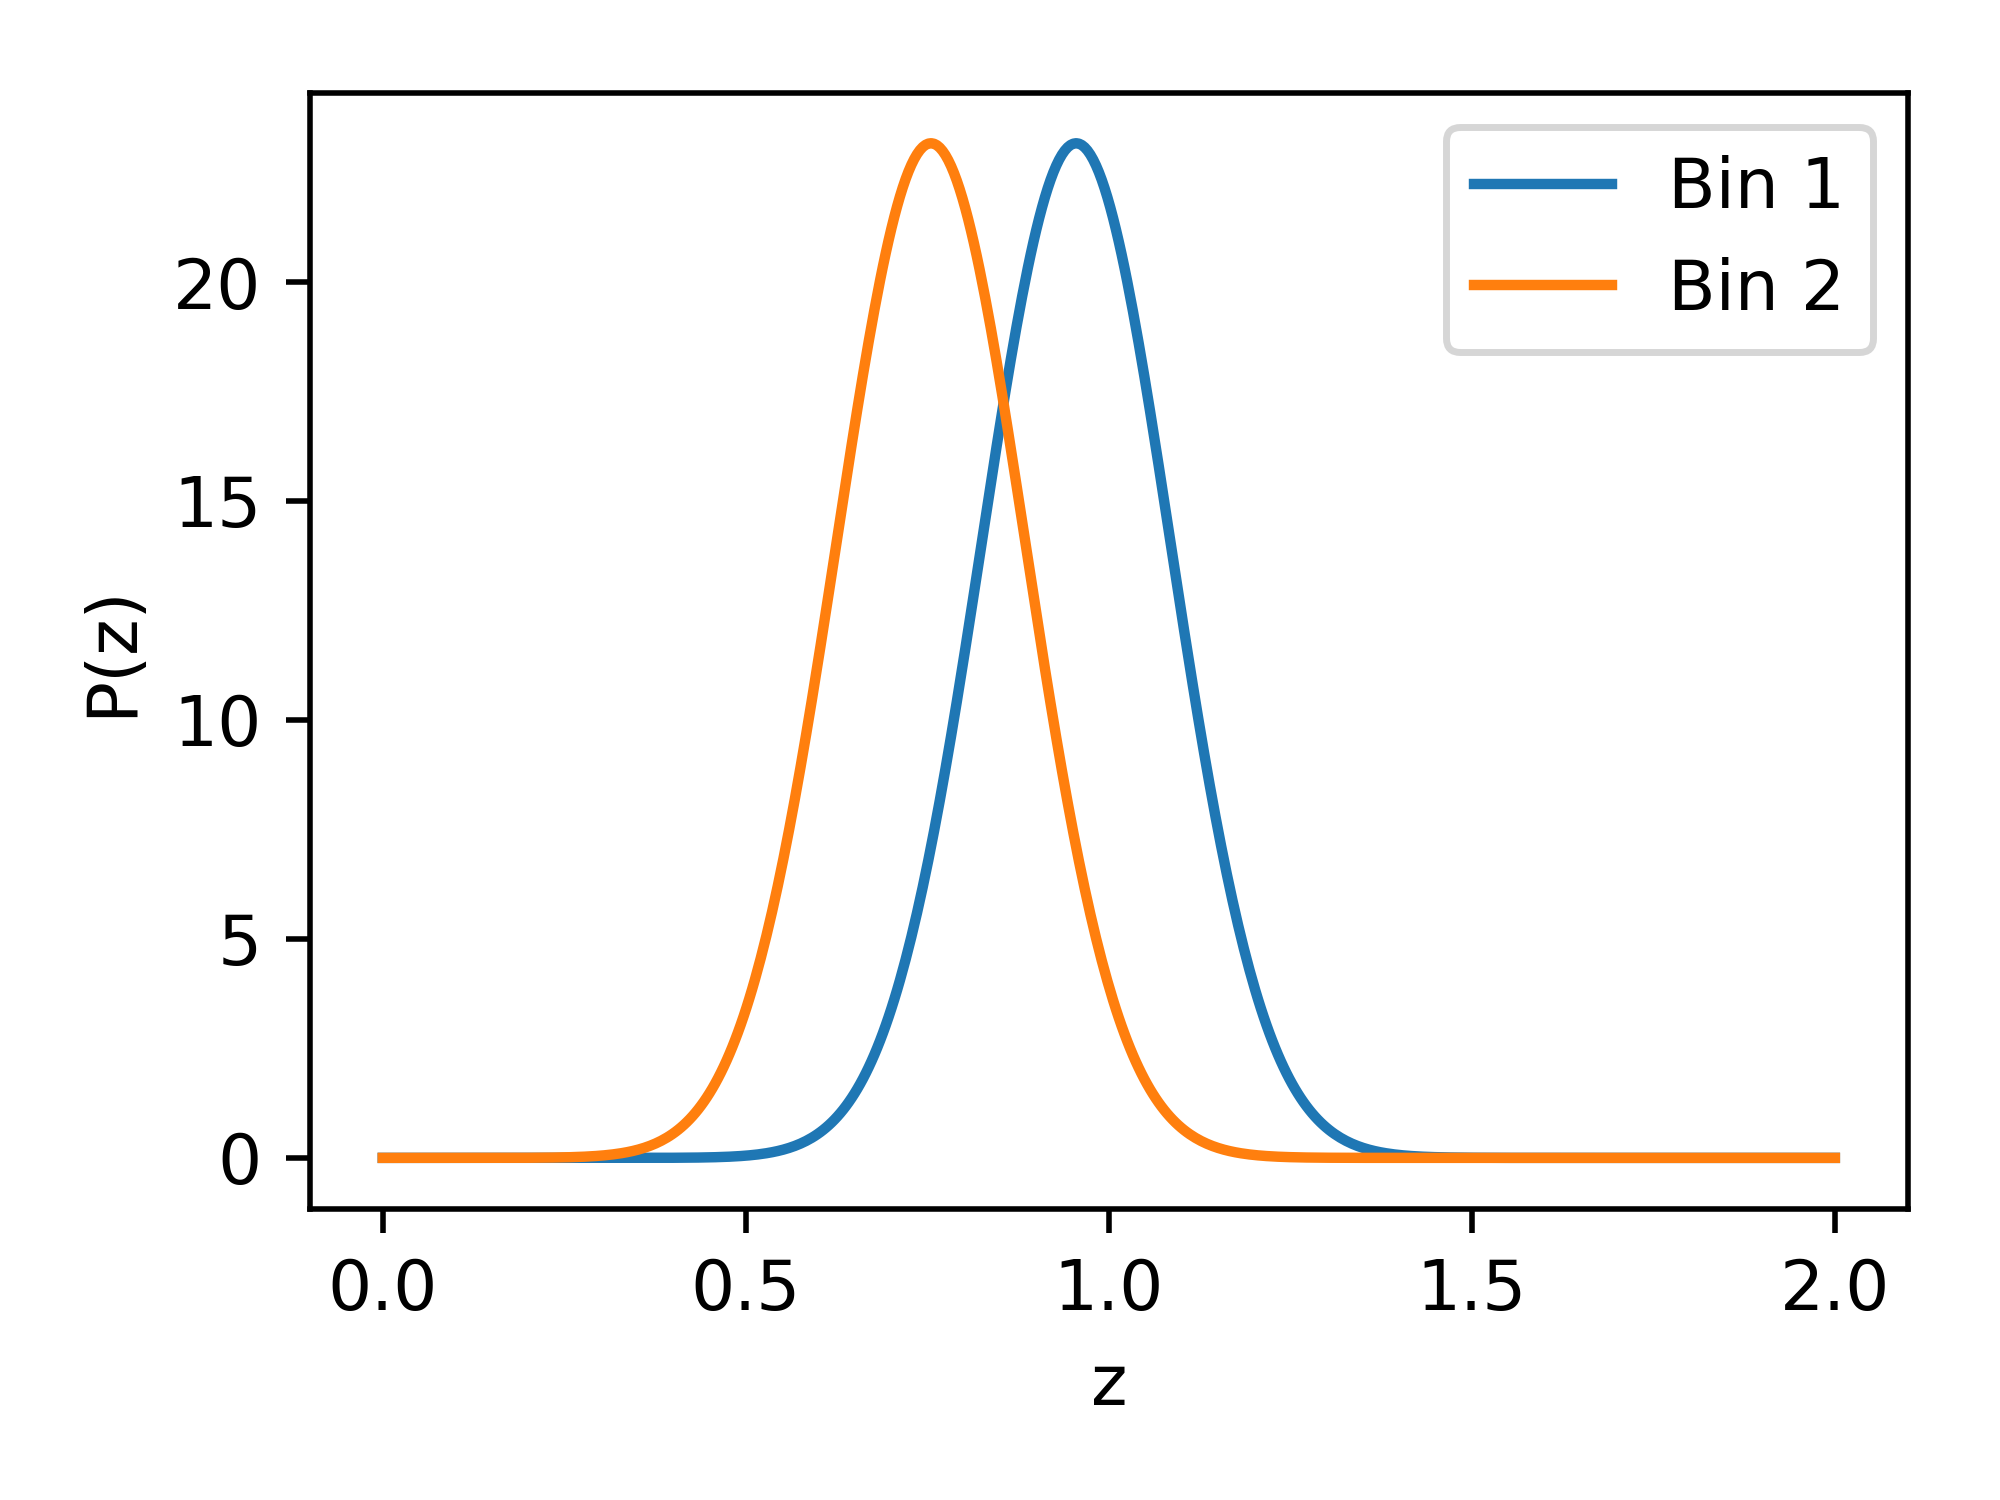
\includegraphics[width=\columnwidth]{./figures/pz.png}
  \caption{Galaxy distribution redshift bins.}
  \label{fig:pz}
\end{figure}

\begin{figure*}
  \centering
  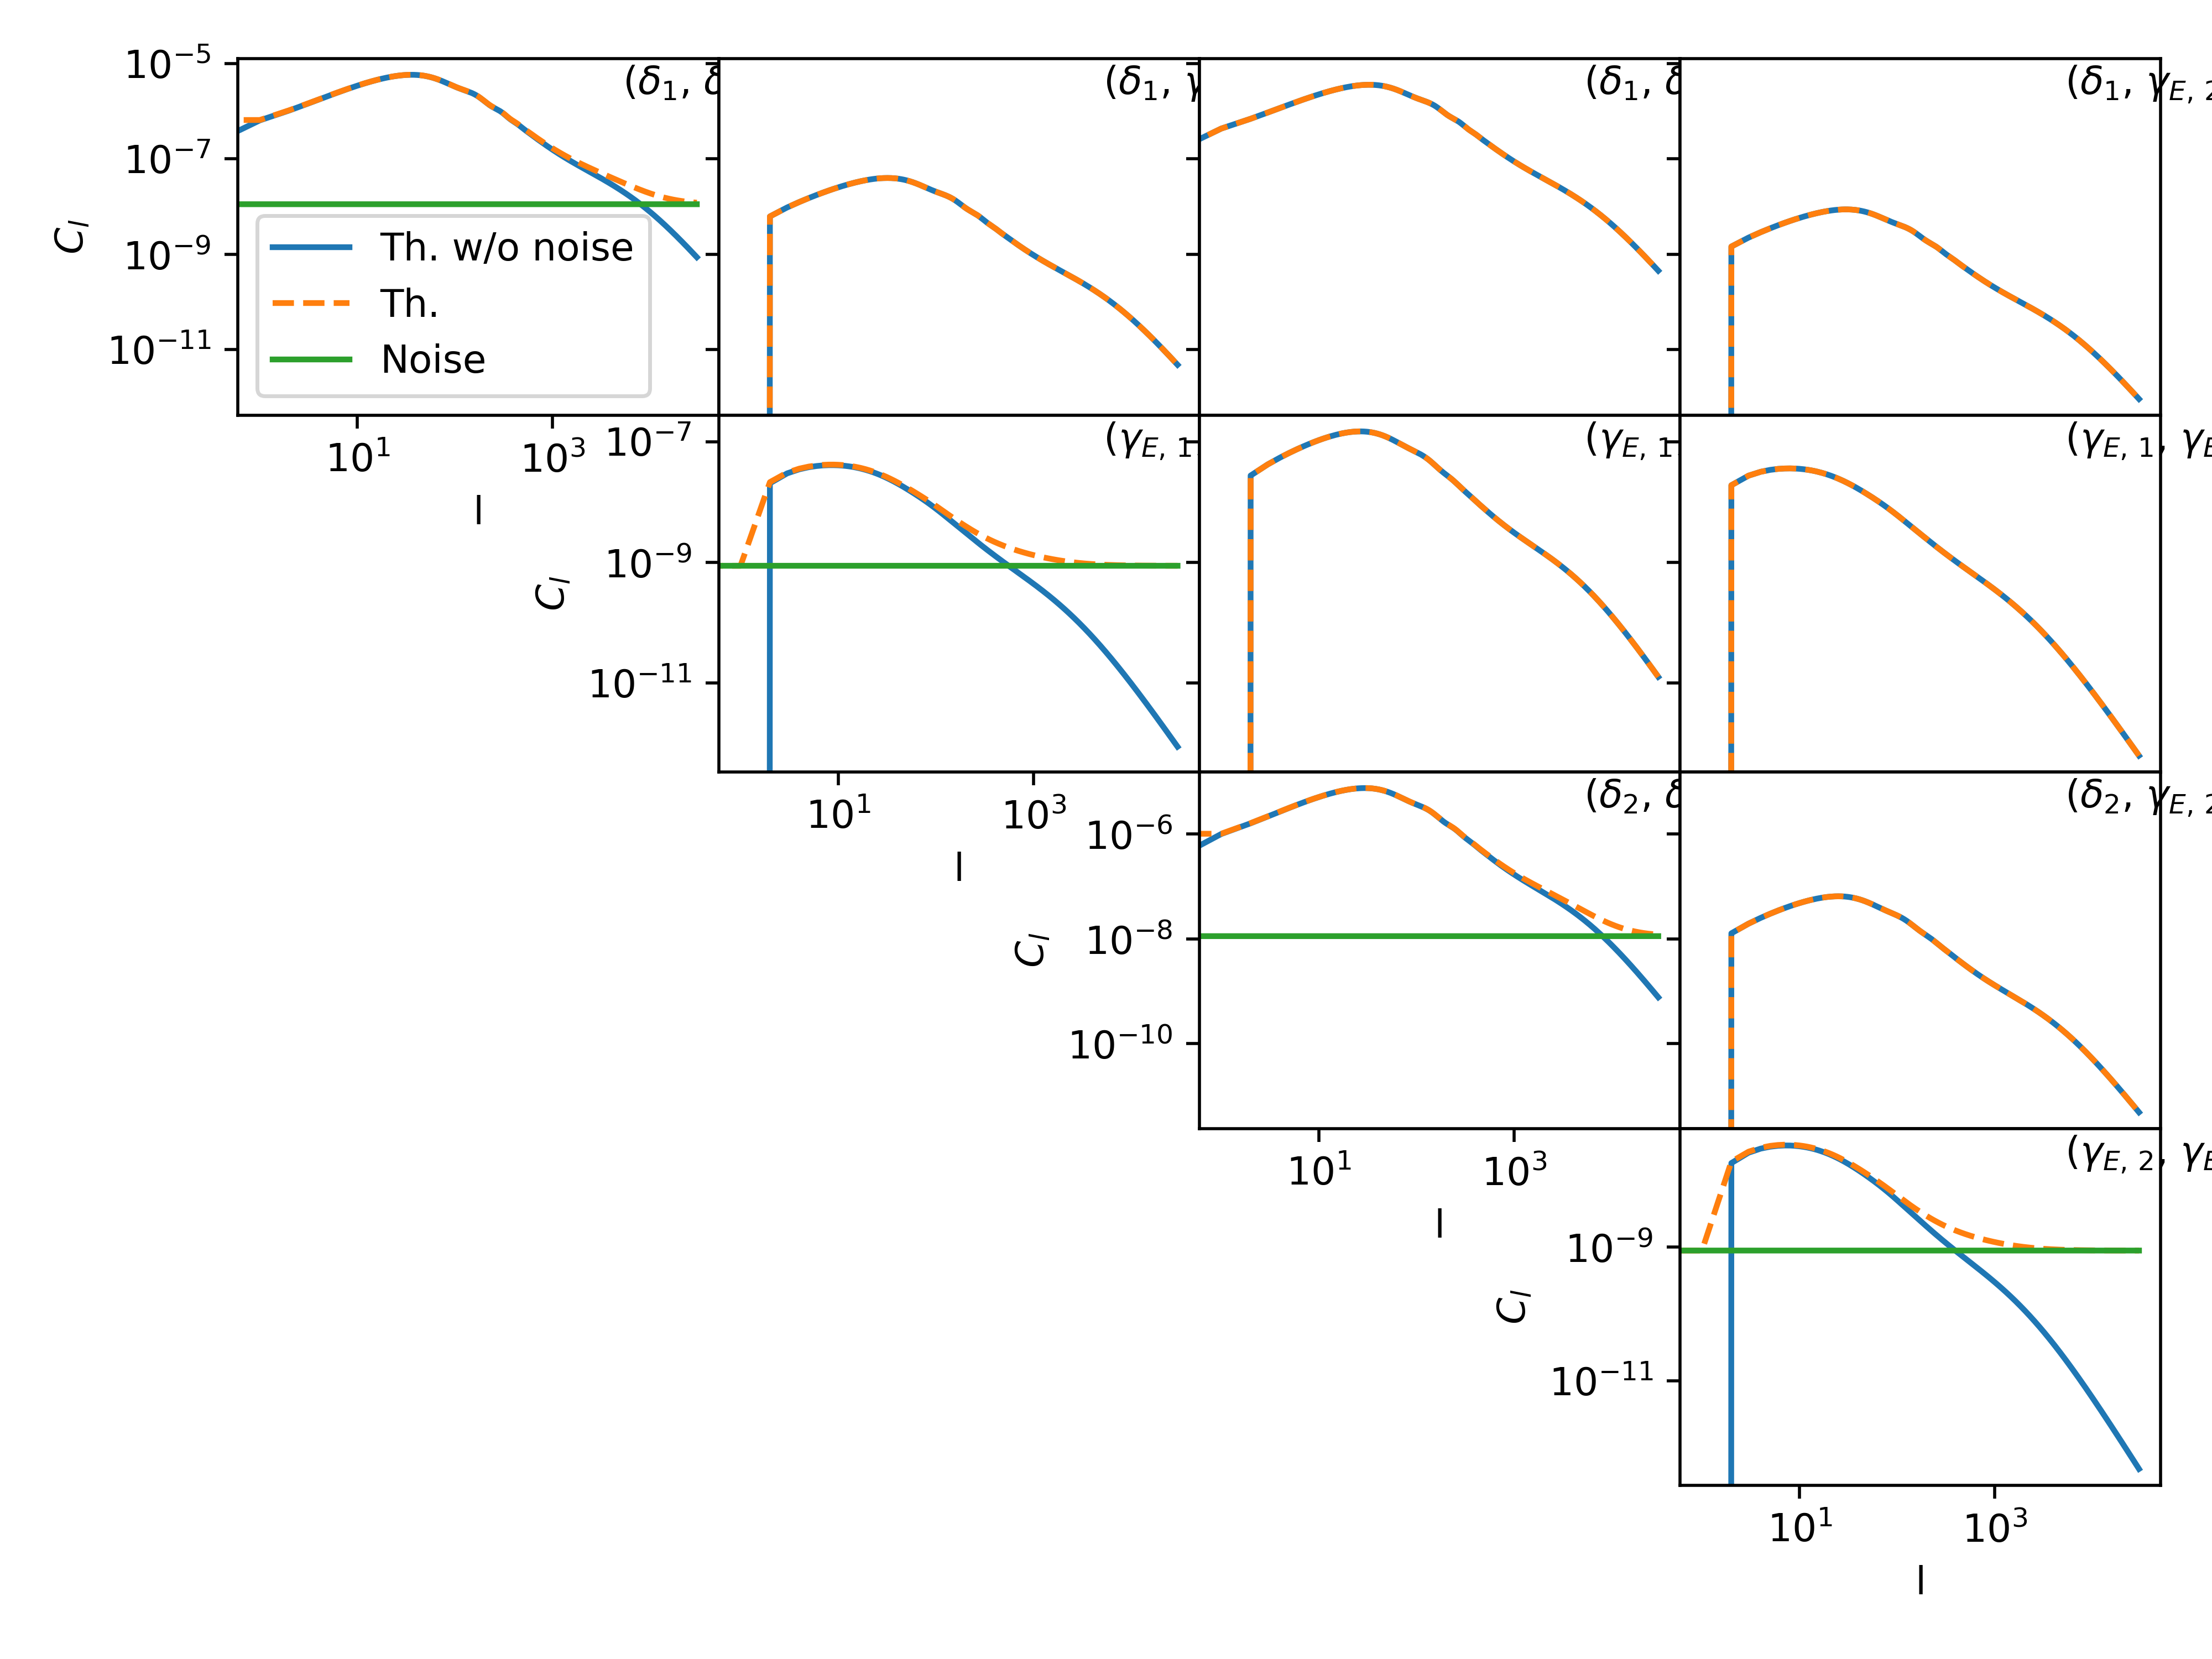
\includegraphics[width=\textwidth]{./figures/cls-sph-2b.png}
  \caption{Fiducial power spectra. We show only the $T$ and $E$ modes.}
  \label{fig:cl-2bins}
\end{figure*}

\begin{figure}
  \centering
  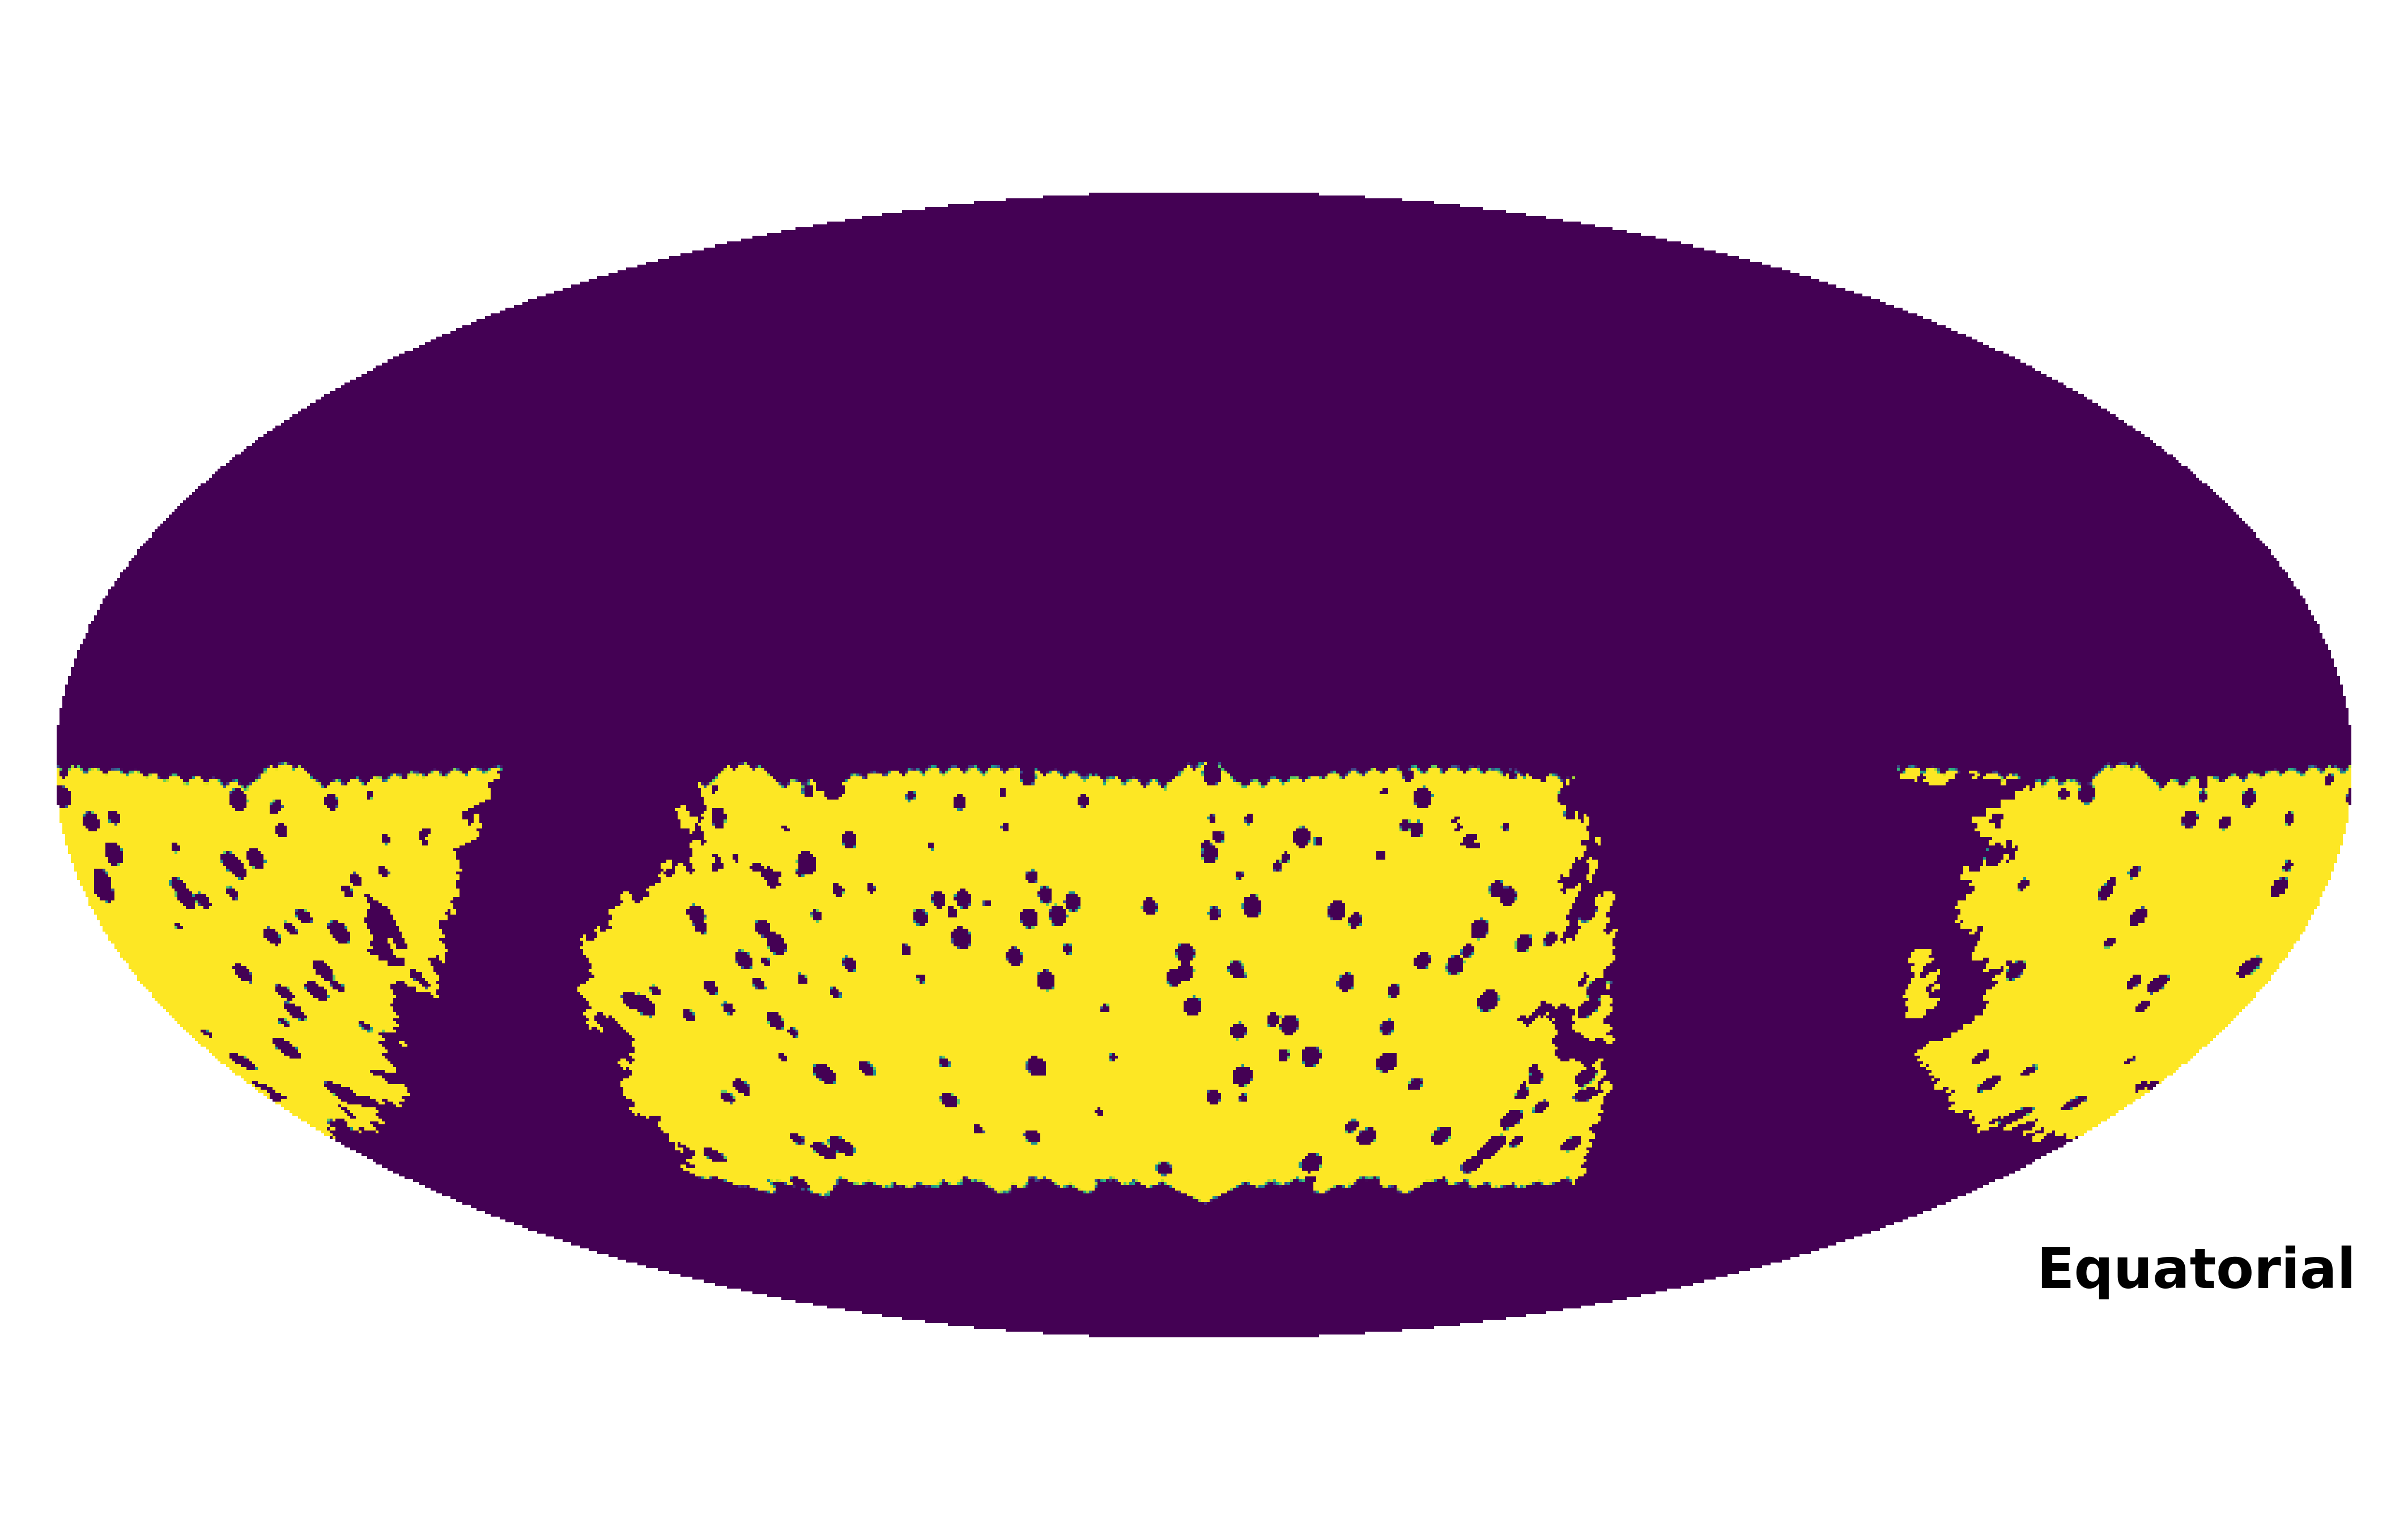
\includegraphics[width=\columnwidth]{./figures/mask-lss1.png}\\
  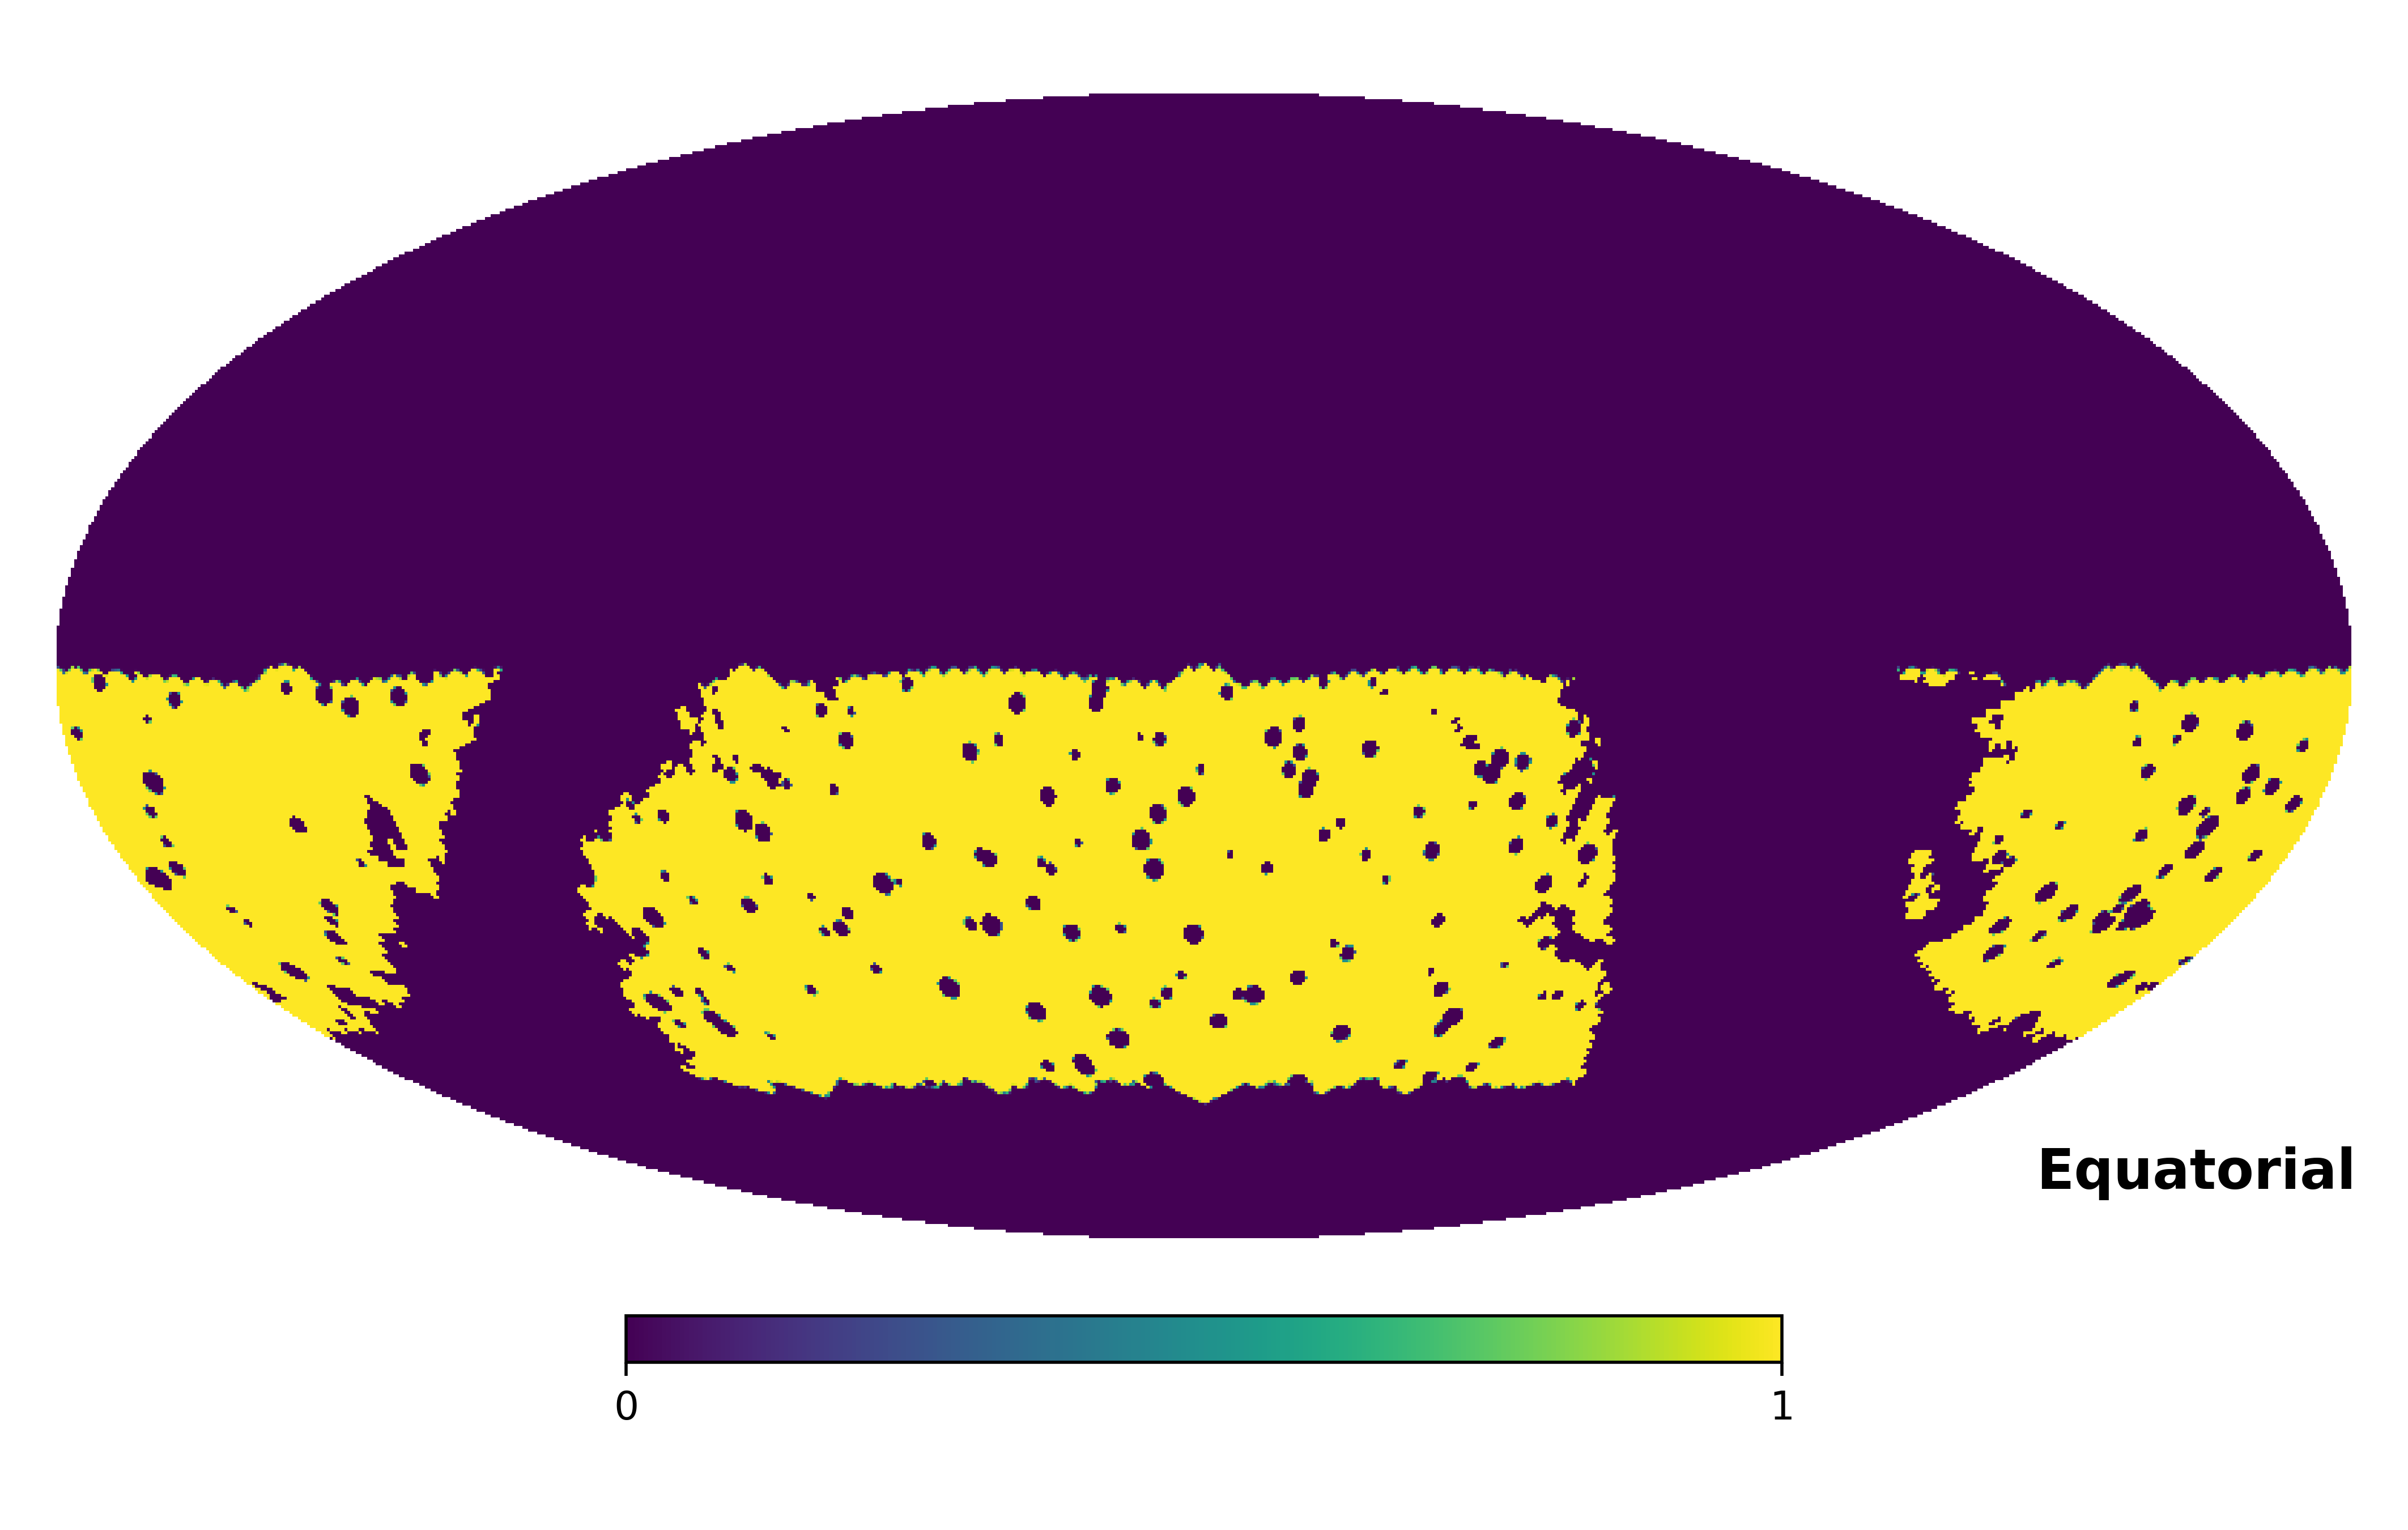
\includegraphics[width=\columnwidth]{./figures/mask-lss2.png}
  \caption{Sky mask used in our analysis}
  \label{fig:mask}
\end{figure}

The covariance matrices were obtained from 20000 simulations, for the band
powers determined by the fraction of sky observed and the maximum band power
we were able to recover the fiducial power spectra for; i.e. $\sim 2 \times
512$. This corresponds to $l_{\mbox{bpw}} = 1023$. To work with the sky
maps and masks we used
\textit{HEALPix}\footnote{\url{https://healpix.jpl.nasa.gov/}}, whereas 
\textit{NaMaster}\footnote{\url{https://github.com/LSSTDESC/NaMaster}}~\cite{2018arXiv180909603A}
was used for the computation of the pseudo-$\cl$ and the covariances. Our code
is publicly
available~\footnote{\url{https://github.com/damonge/PCLCovariance}}.

The same results are obtained even in the presence of foregrounds. In
particular, we tested the case with 100 foregrounds both at low scales and
large scales, adding a mock power spectra (e.g. Fig.~\ref{fig:fore}) computed as 
\begin{equation}
  \clf = A (l + 1)^{\beta}\,.
  \label{eq:fore}
\end{equation}
Here, $A$ was fixed so that the ratio of the foreground power spectra and the
theoretical one ($\clth$) was $\clf/\clth = 0.1$ at $l=400$ and $\beta$ was
randomly chosen from $U[-3, -1)$ for large scale effects and fixed to $\beta =
0$ for small scale ones. 

\begin{figure}
  \centering
  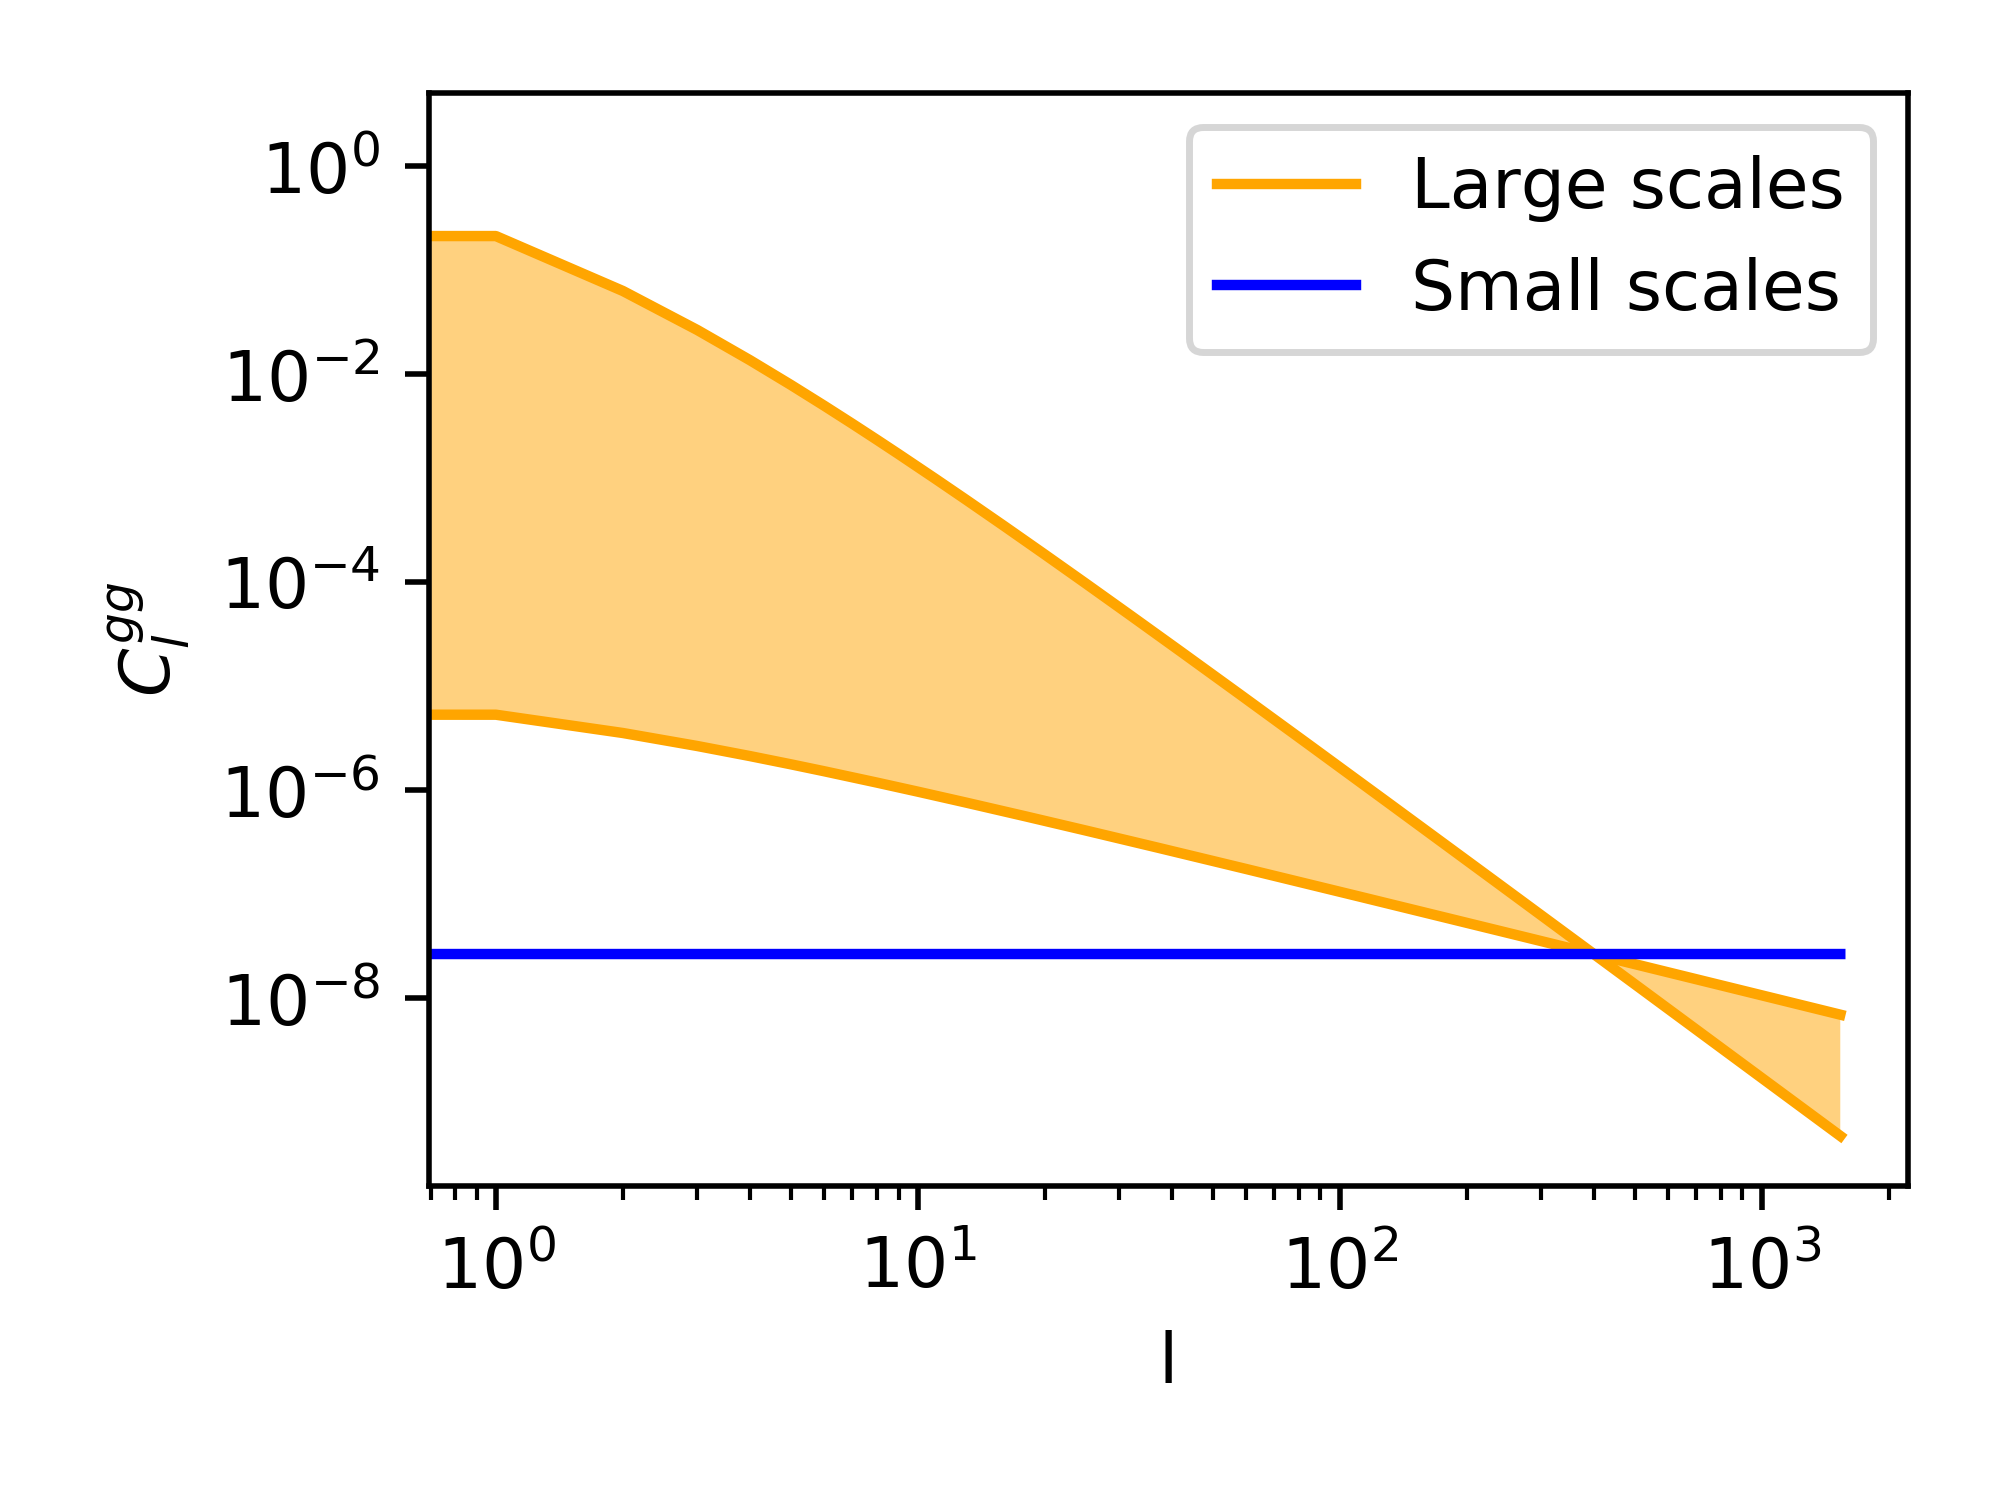
\includegraphics[width=\columnwidth]{./figures/foreground.png}
  \caption{$\cl$ foregrounds used in order to check the reliability of the
    analytical approximations in their presence. They did not affect. The
    limiting cases for the large-scale contaminants are given by $\beta=-1,\,
    -3$ in Eq.~\ref{eq:fore}}
  \label{fig:fore}
\end{figure}

\subsection{Visual inspection}
\todo{Rows plot para todas las combinaciones}
\todo{diff-correlation TTTT BBBB}
\todo{Eigenvalue plot}

\subsection{Quantitative checks}
\todo{Plot $\chi^2$ TT-TT, TE-TE, EE-EE}

\subsection{Contaminant deprojection}
\todo{}

\subsection{Impact on parameter estimation}
\todo{$\chi^2$ plot para 2 bines}
\todo{diff-correlaton plot para 2 bines ver Fig. 8  de 1809.09603}
\todo{Contours}

\subsection{$\chi^2$ distribution and covariance matrices - old section}
Apart from checking that we recover the same cosmological predictions from the
covariance matrices from both the analytical approximation and the
simulations, we studied the differences between them.

In this sense, one can see in Fig.~\ref{fig:TTTT_EEEE_chi2} that, we fully
recover the $\chi^2$ distribution (defining $\chi^2 = \cl - \langle \cl
\rangle C^{-1} \cl - \langle \cl \rangle$) for the TTTT case; whereas for the
worst case (i.e. EEEE) we are able to recover its shape, although sifted
toward lower values. This might be consequence of the fact that the inverse of
the covariance matrix is biased. It is interesting to note that even
the approximation of the mixing matrix as that of the case with spin 0, gives
good results. The eigenvalues of the covariance matrix
(Fig.~\ref{fig:TTTT_EEEE_eigv}) are also recovered within the 1\%, for all
scales in the TTTT case, and for the smaller scales in the EEEE case. Finally,
the analytical approximations are shown to describe the scale coupling (see
Fig.~\ref{fig:TTTT_rows} that comes from the fact we are masking some regions
of the sky. The larger relative deviation for the better approximations are
due to the fact that there is a division by $0$, while for the naive
approximation, which is defined diagonal (see Eq.~\ref{eq:naive}), the
relative deviation is exactly $-1$ for all values with $l \neq l'$.

\begin{figure*} %[htb]
  \centering
  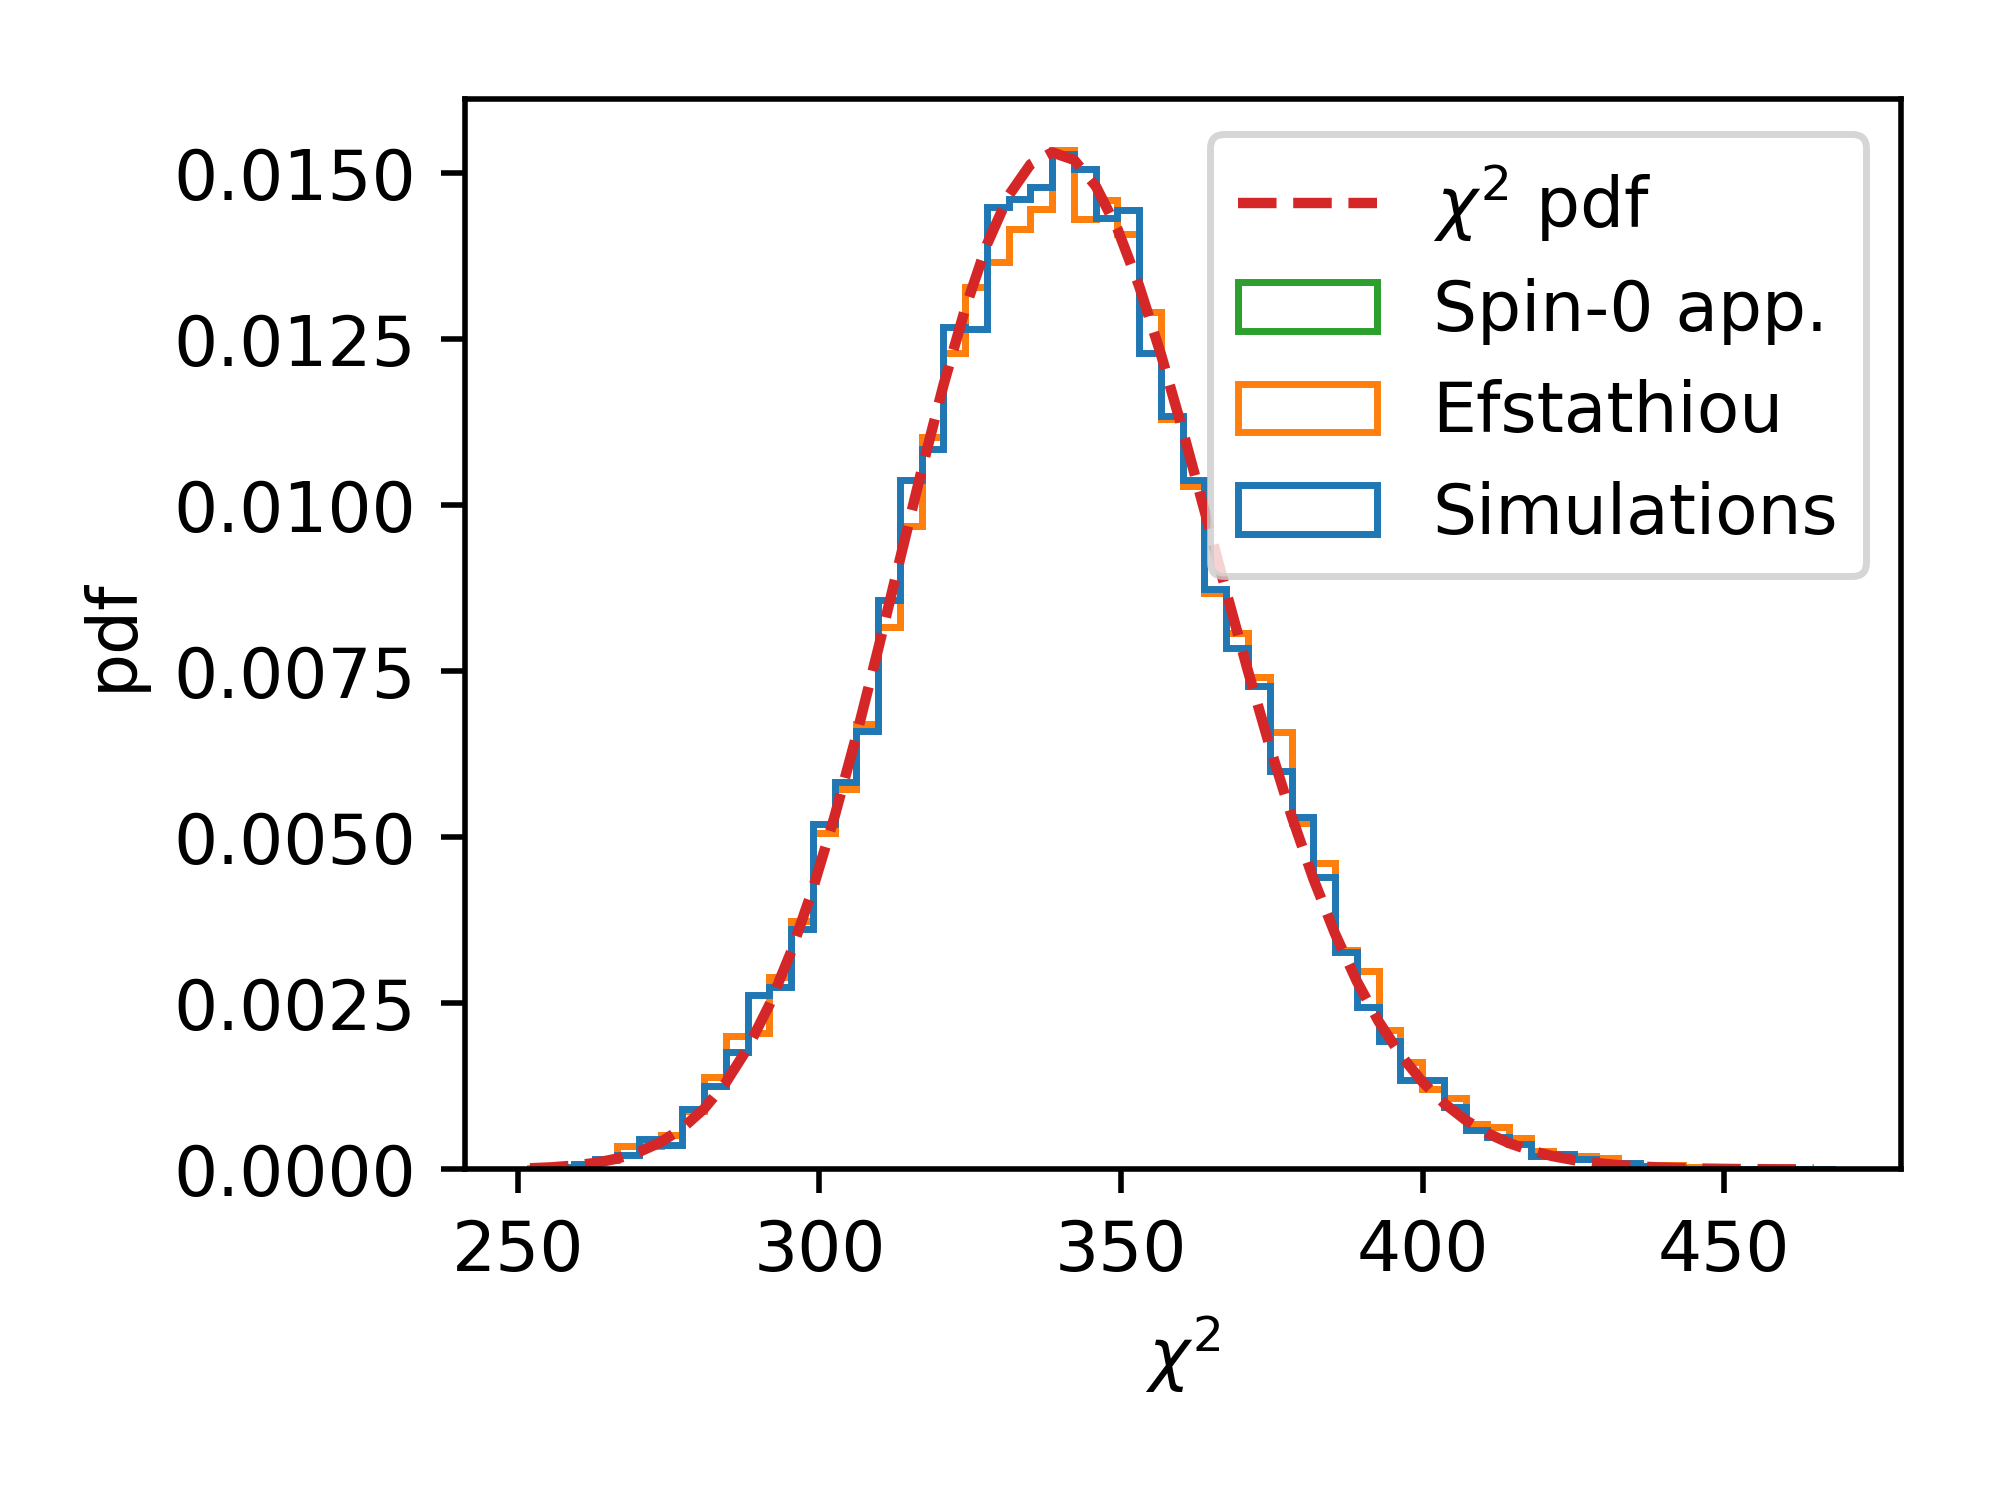
\includegraphics[width=\columnwidth]{./figures/run_sph_ALL_TTTT_chi2.png}~
  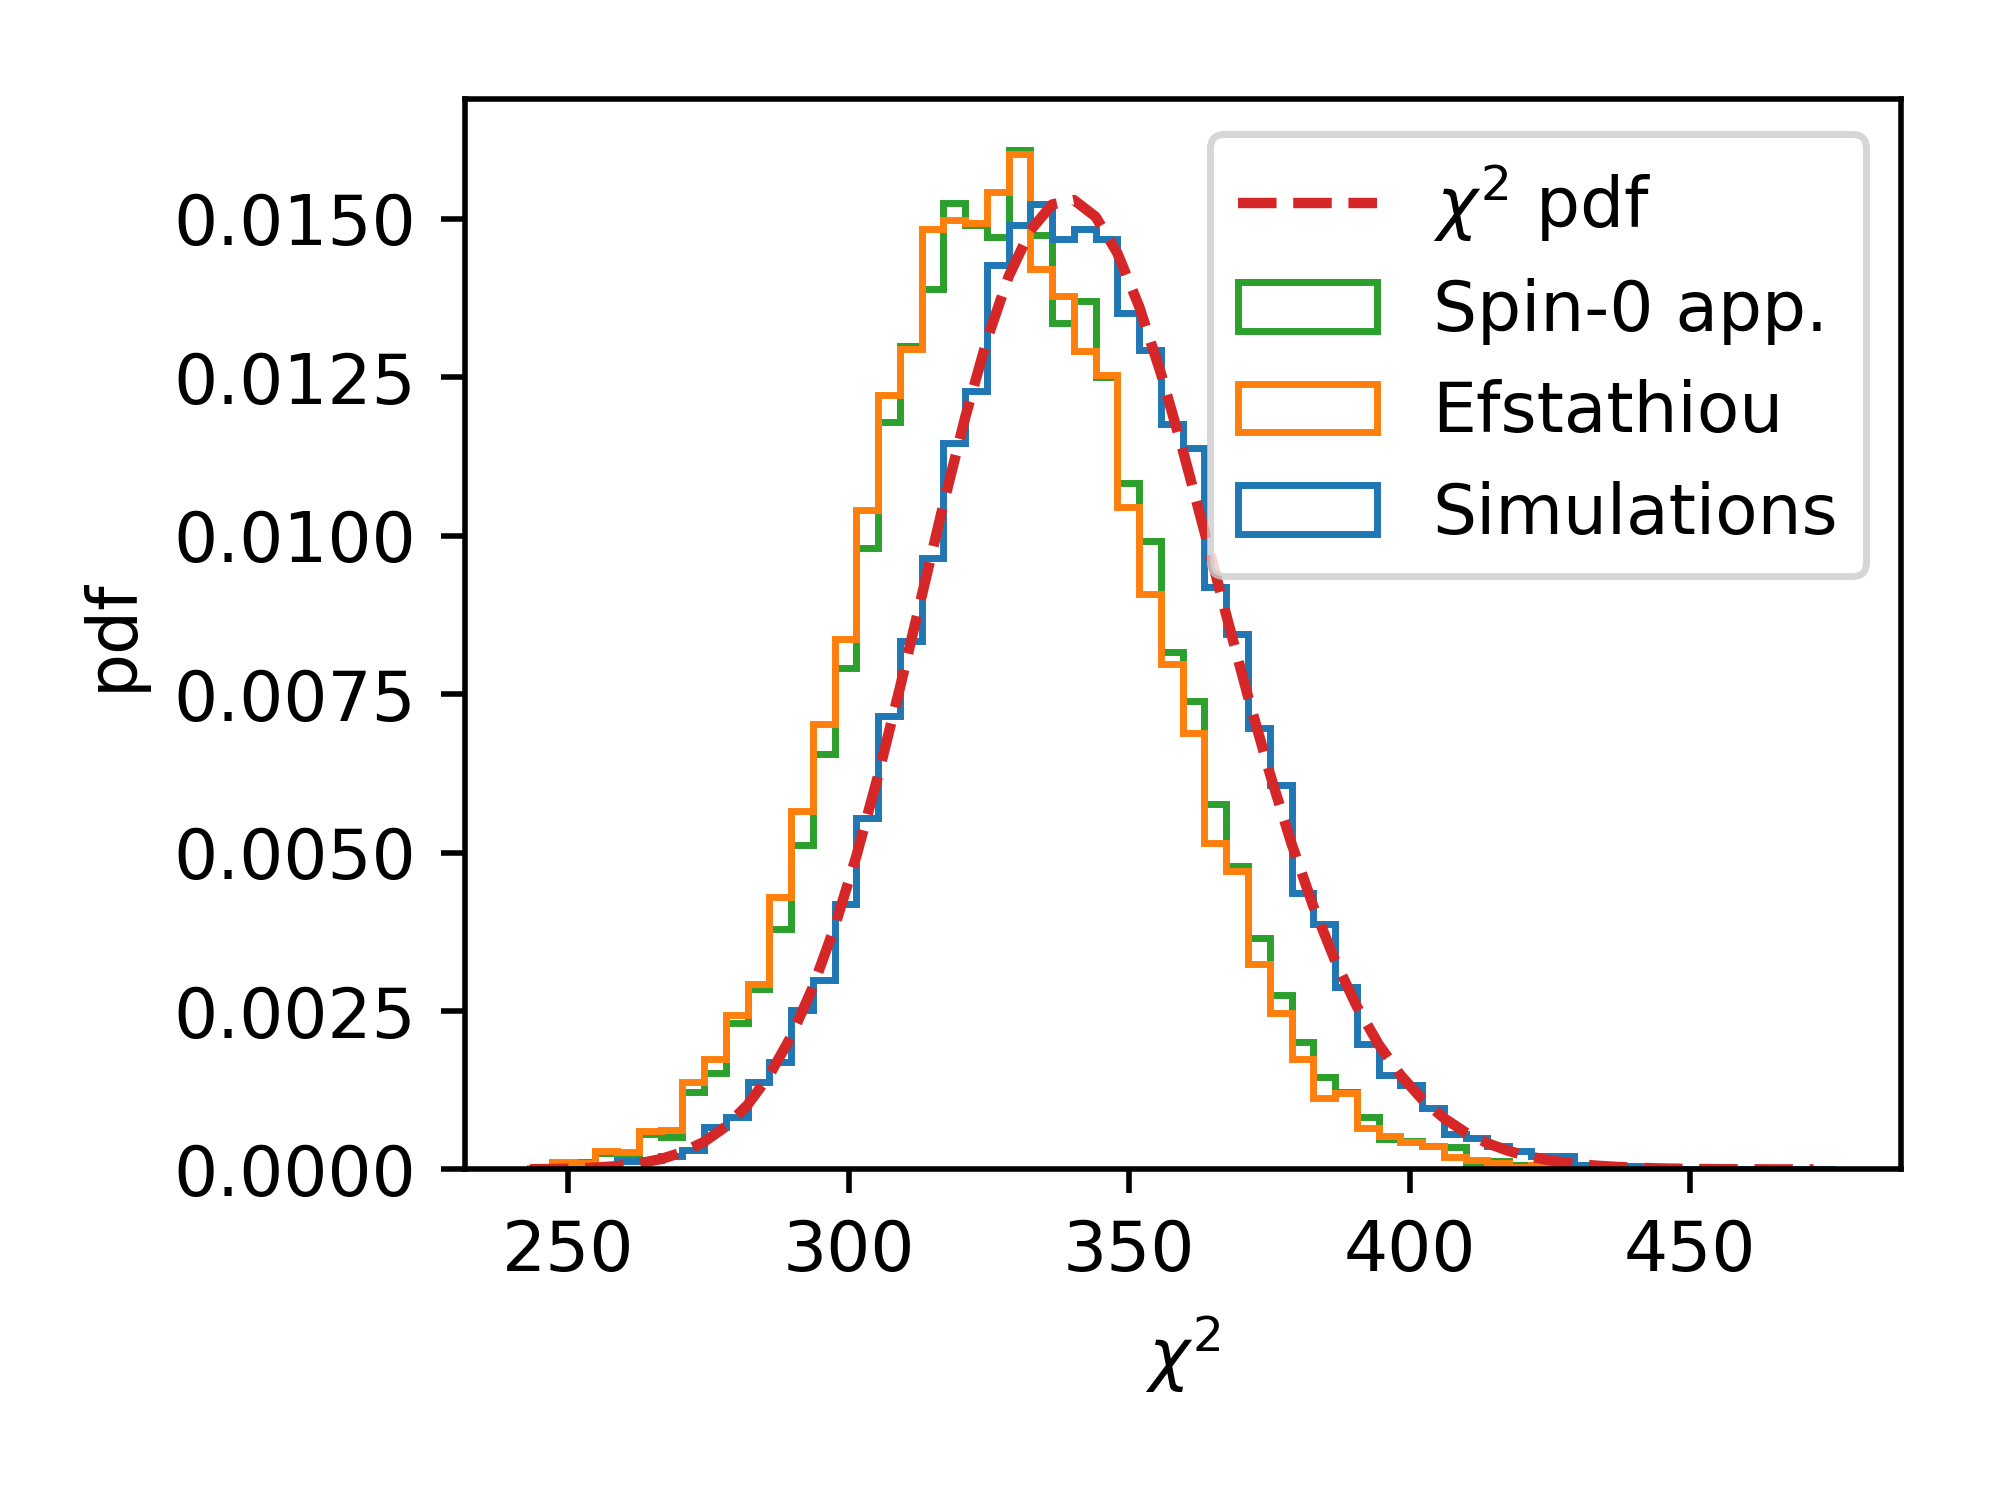
\includegraphics[width=\columnwidth]{./figures/run_sph_ALL_EEEE_chi2.png}
  \caption{Comparison of the distributions found using different
    covariances for the TTTT (left) and EEEE (right) cases.}
  \label{fig:TTTT_EEEE_chi2}
\end{figure*}

\begin{figure*} %[htb]
  \centering
  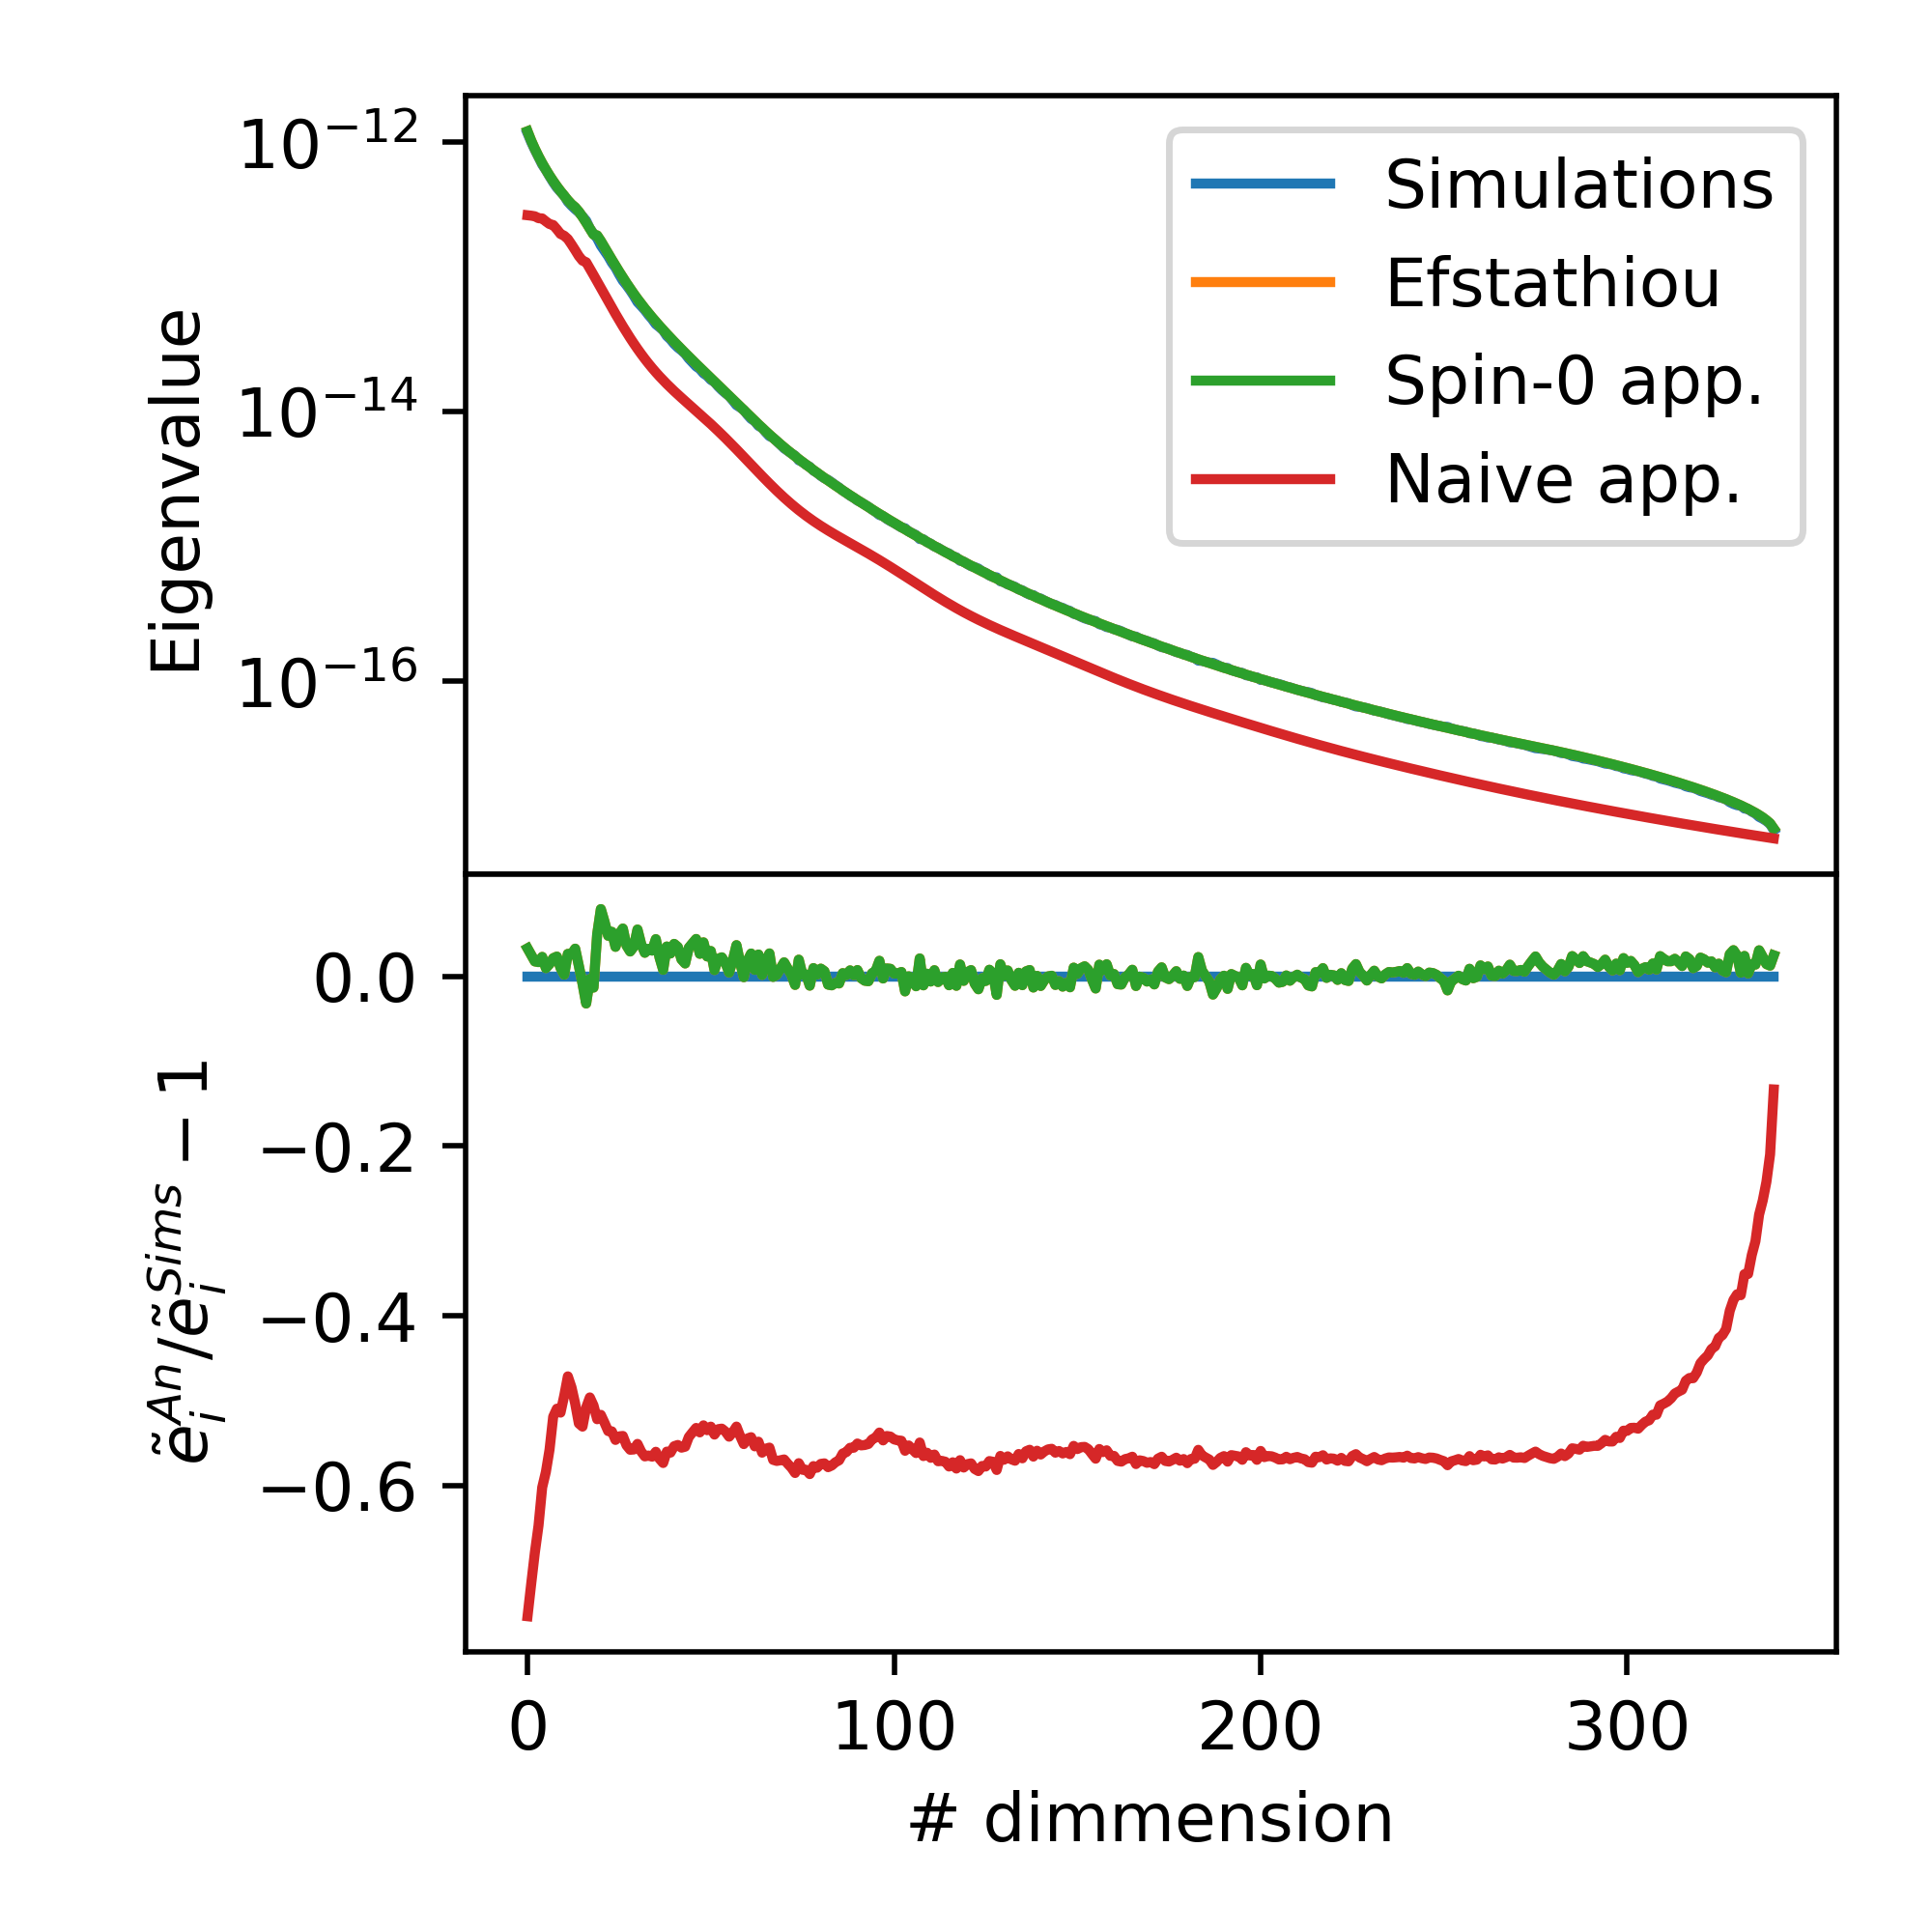
\includegraphics[width=\columnwidth]{./figures/run_sph_ALL_TTTT_reldev_eigval.png}~
  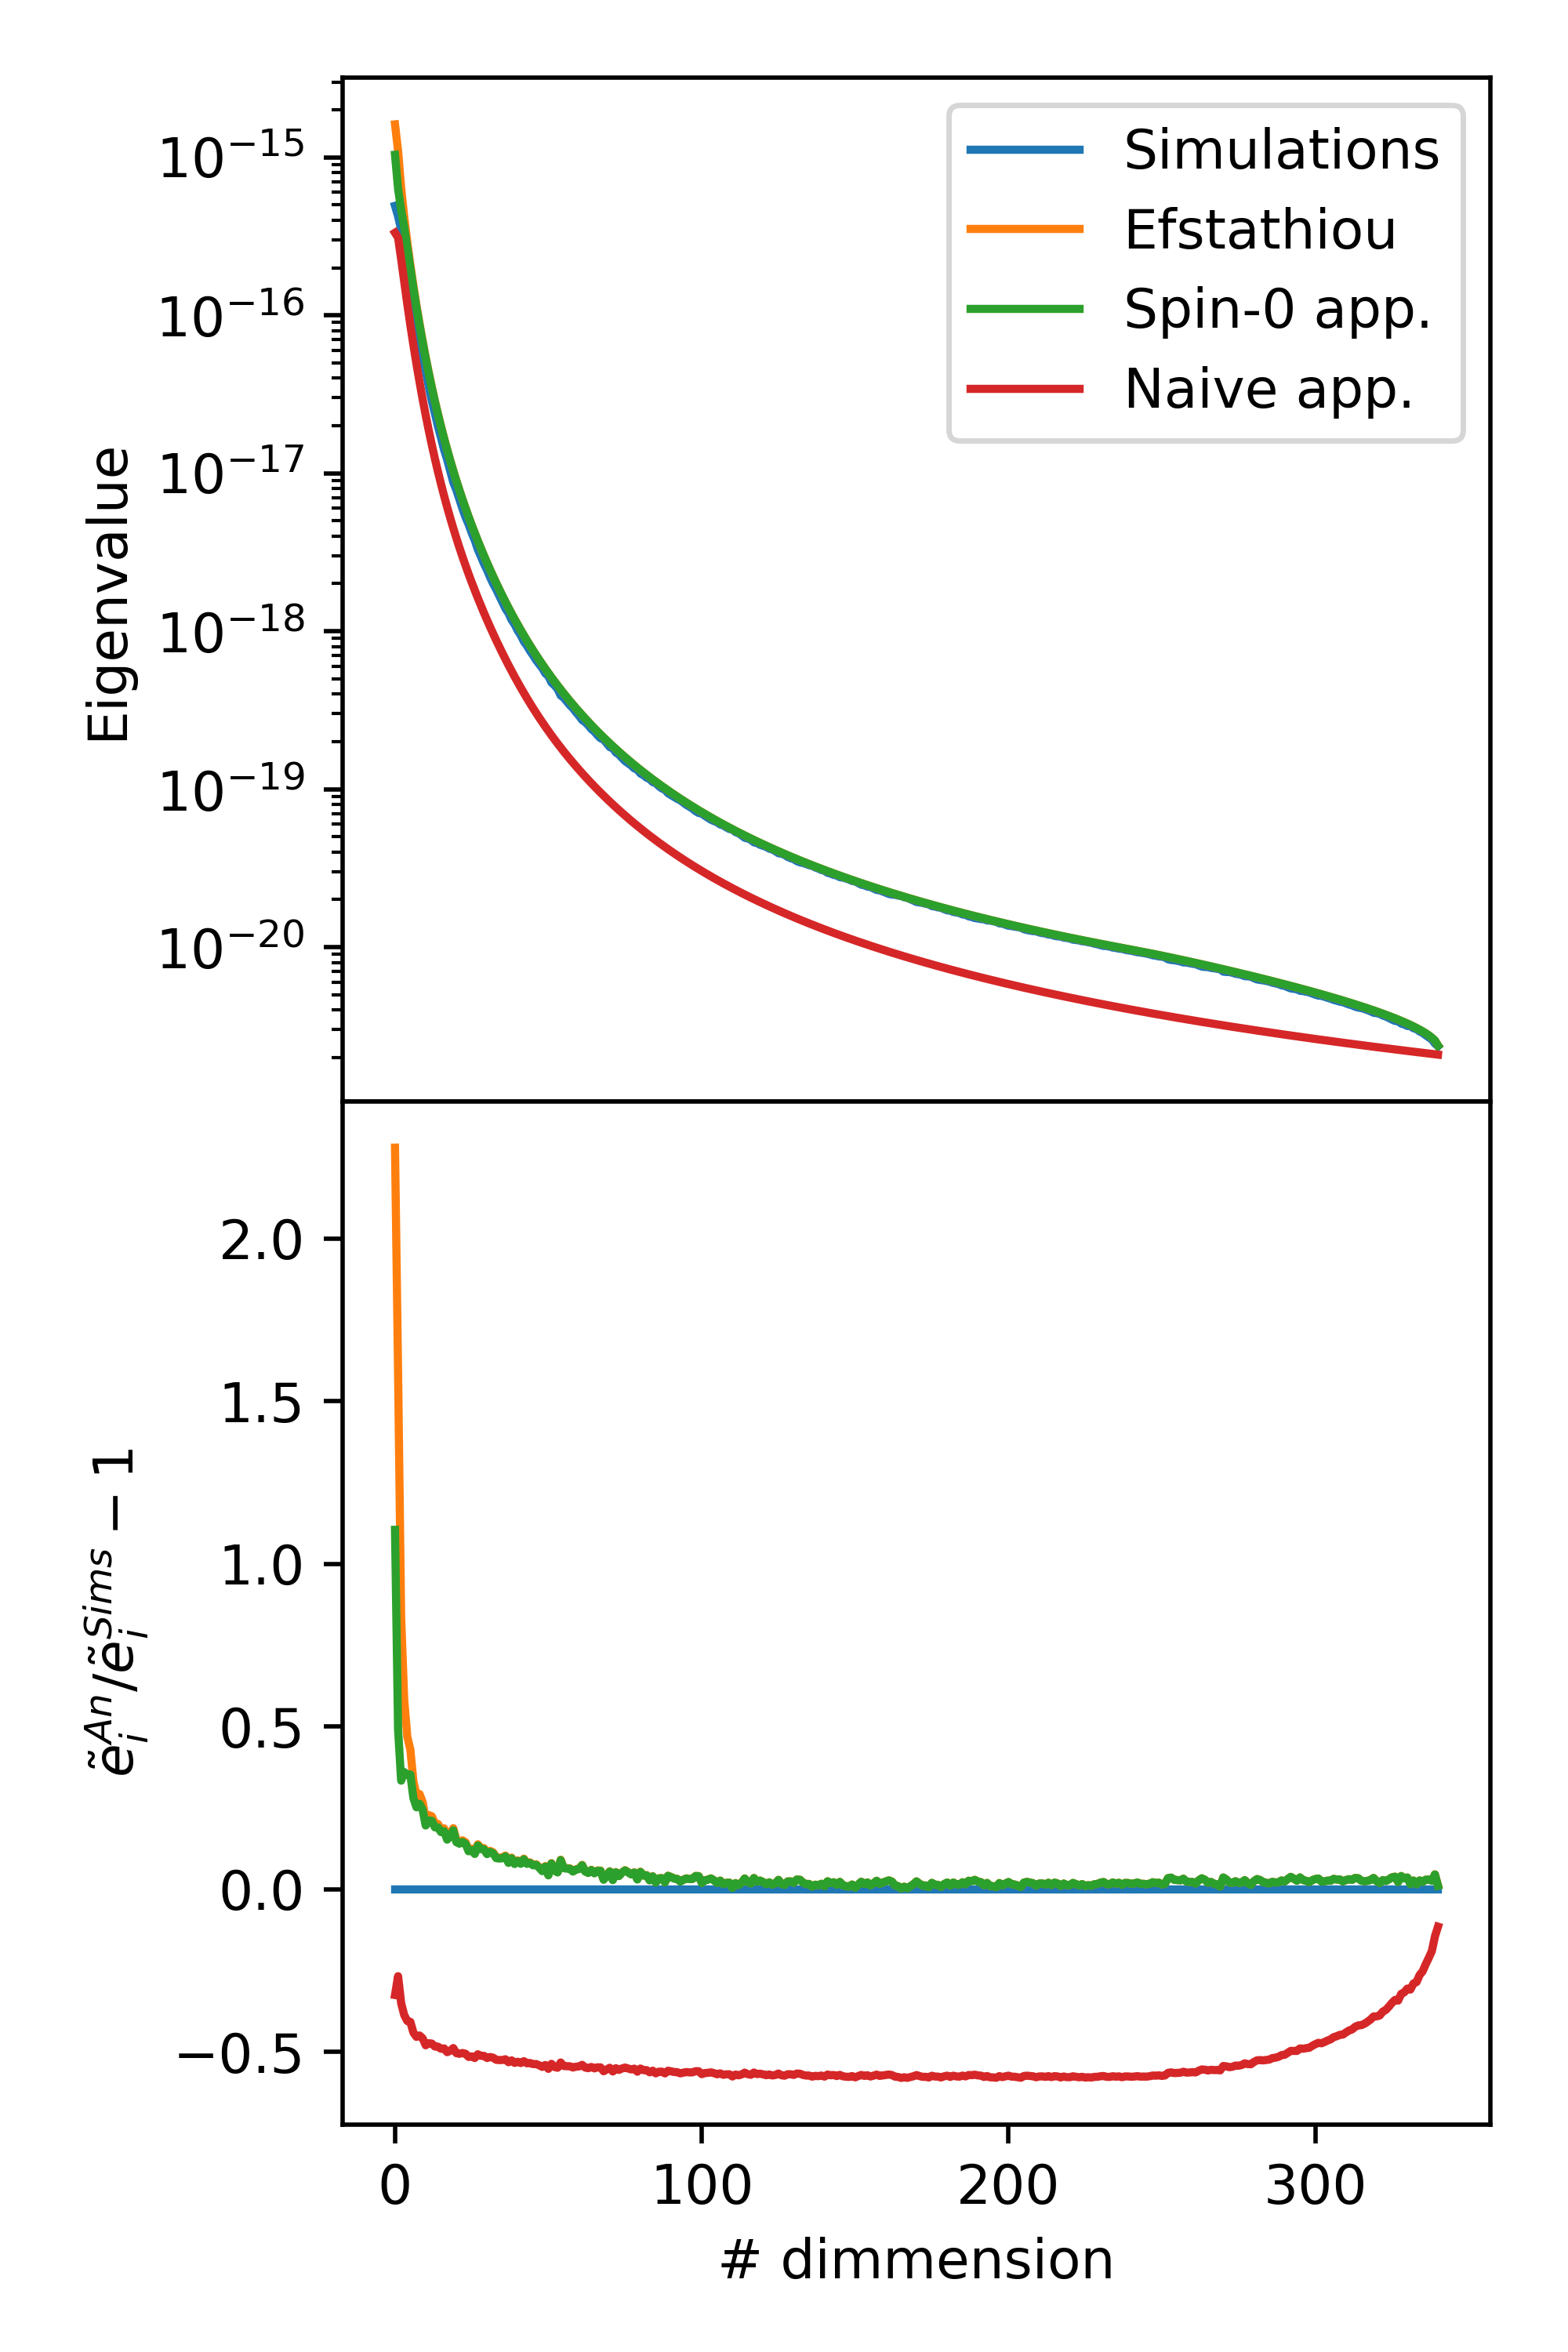
\includegraphics[width=\columnwidth]{./figures/run_sph_ALL_EEEE_reldev_eigval.png}
  \caption{Comparison of the covariance matrix eigenvalues for the TTTT (left)
    and EEEE (right) cases.} 
  \label{fig:TTTT_EEEE_eigv}
\end{figure*}

\begin{figure} %[htb]
  \centering
  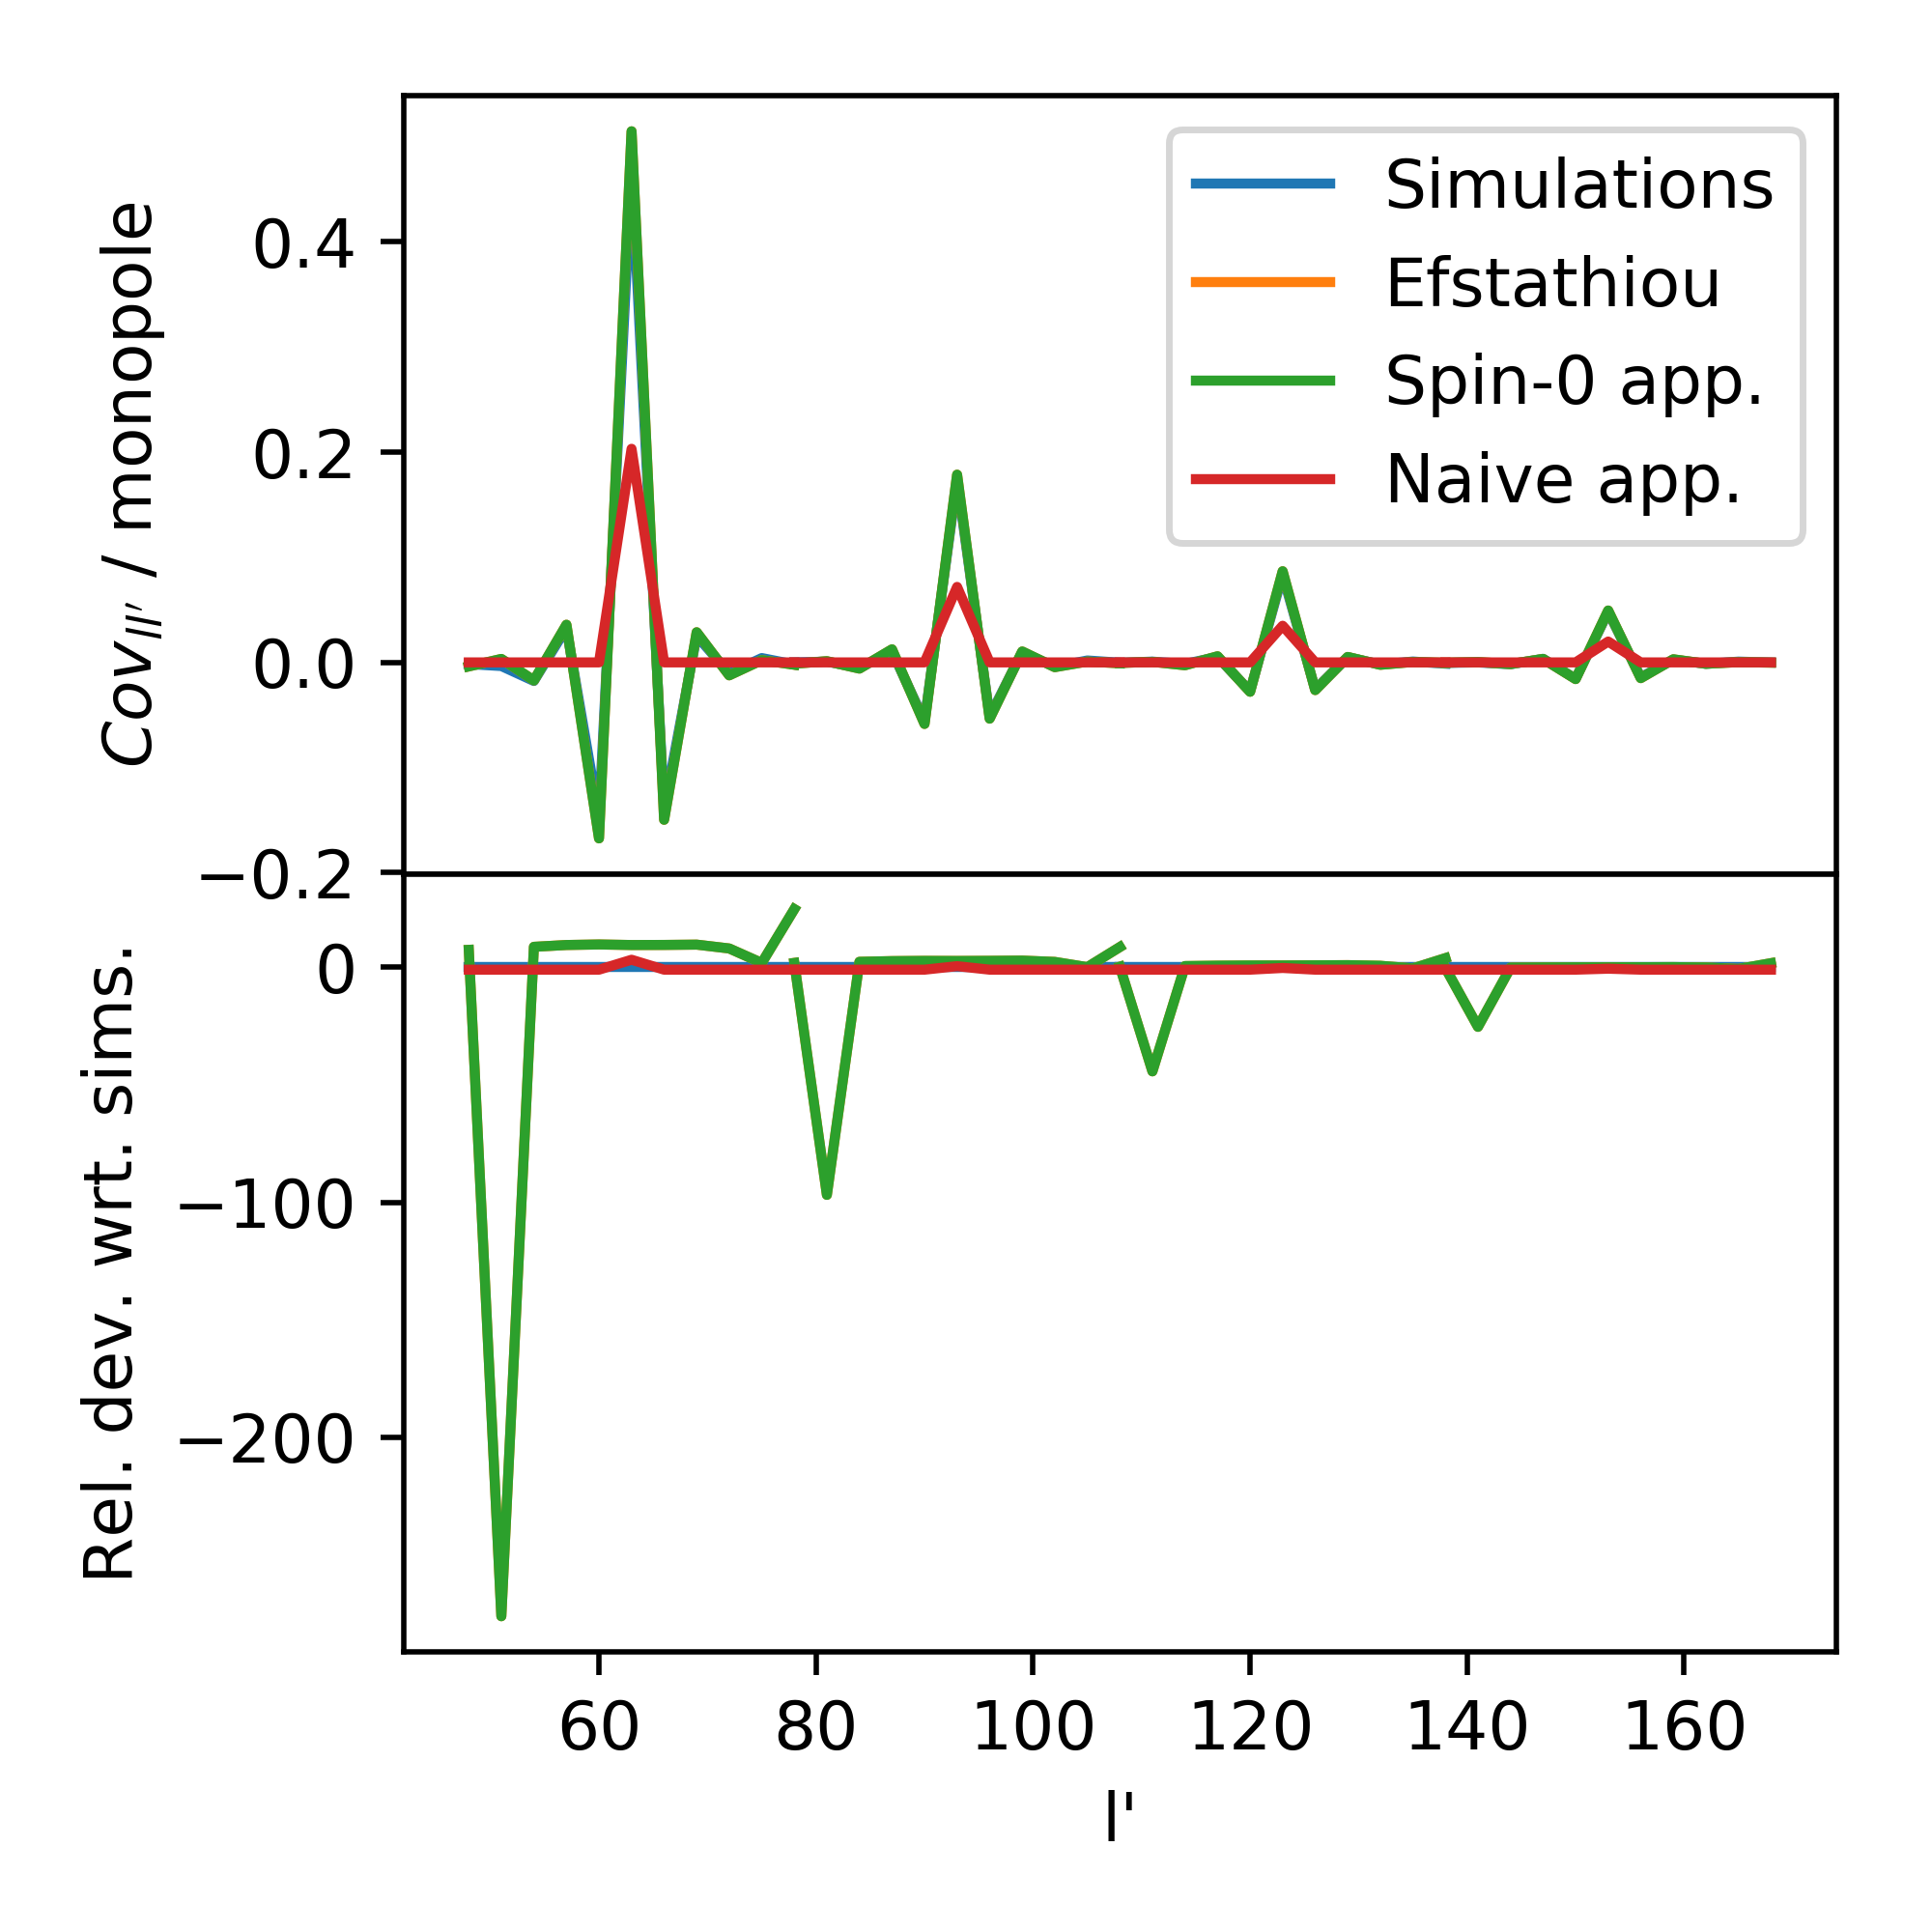
\includegraphics[width=\columnwidth]{./figures/run_sph_ALL_TTTT_rows_cov_matrix.png}~
  \caption{Mask induced scale correlations for the TTTT case.}
  \label{fig:TTTT_rows}
\end{figure}

The goodness of the approximation is also seen in the correlation matrices.
The subtraction of the correlation matrix from the simulations and that from
the best analytical approximation (which we have just seen gives almost same
results as the spin-0 one) shows no structure but for the case of the larger
scales of the EEEE modes (see Fig.~\ref{fig:TTTT_EEEE_corr}).

\begin{figure*} %[htb]
  \centering
  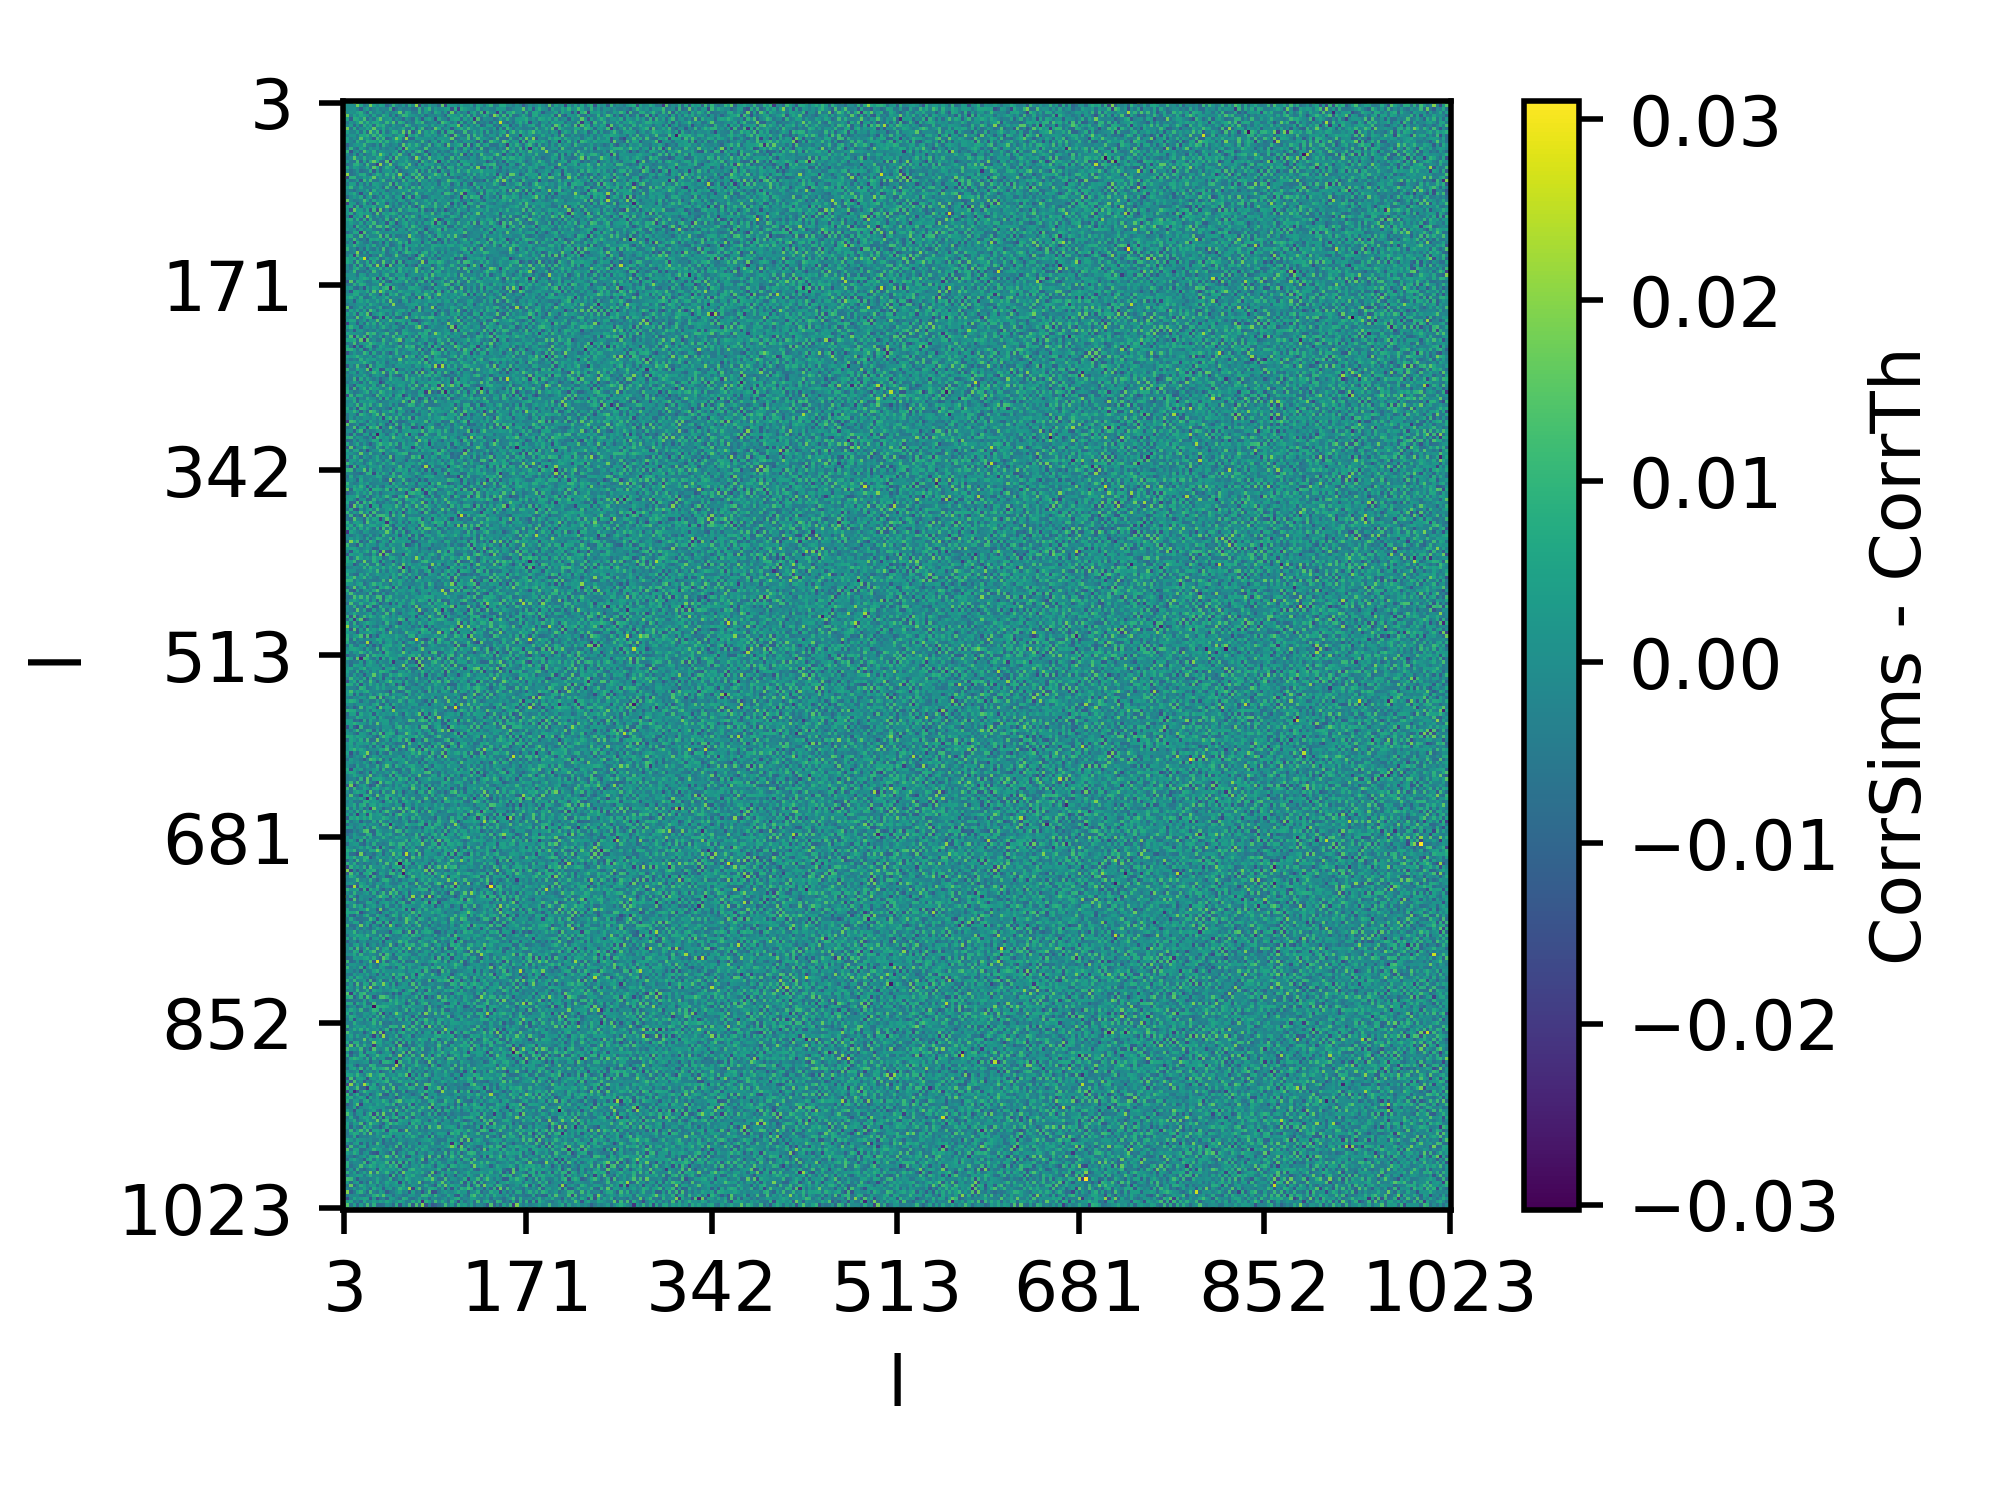
\includegraphics[width=\columnwidth]{./figures/run_sph_Efstathiou_TTTT_correlation_difference.png}~
  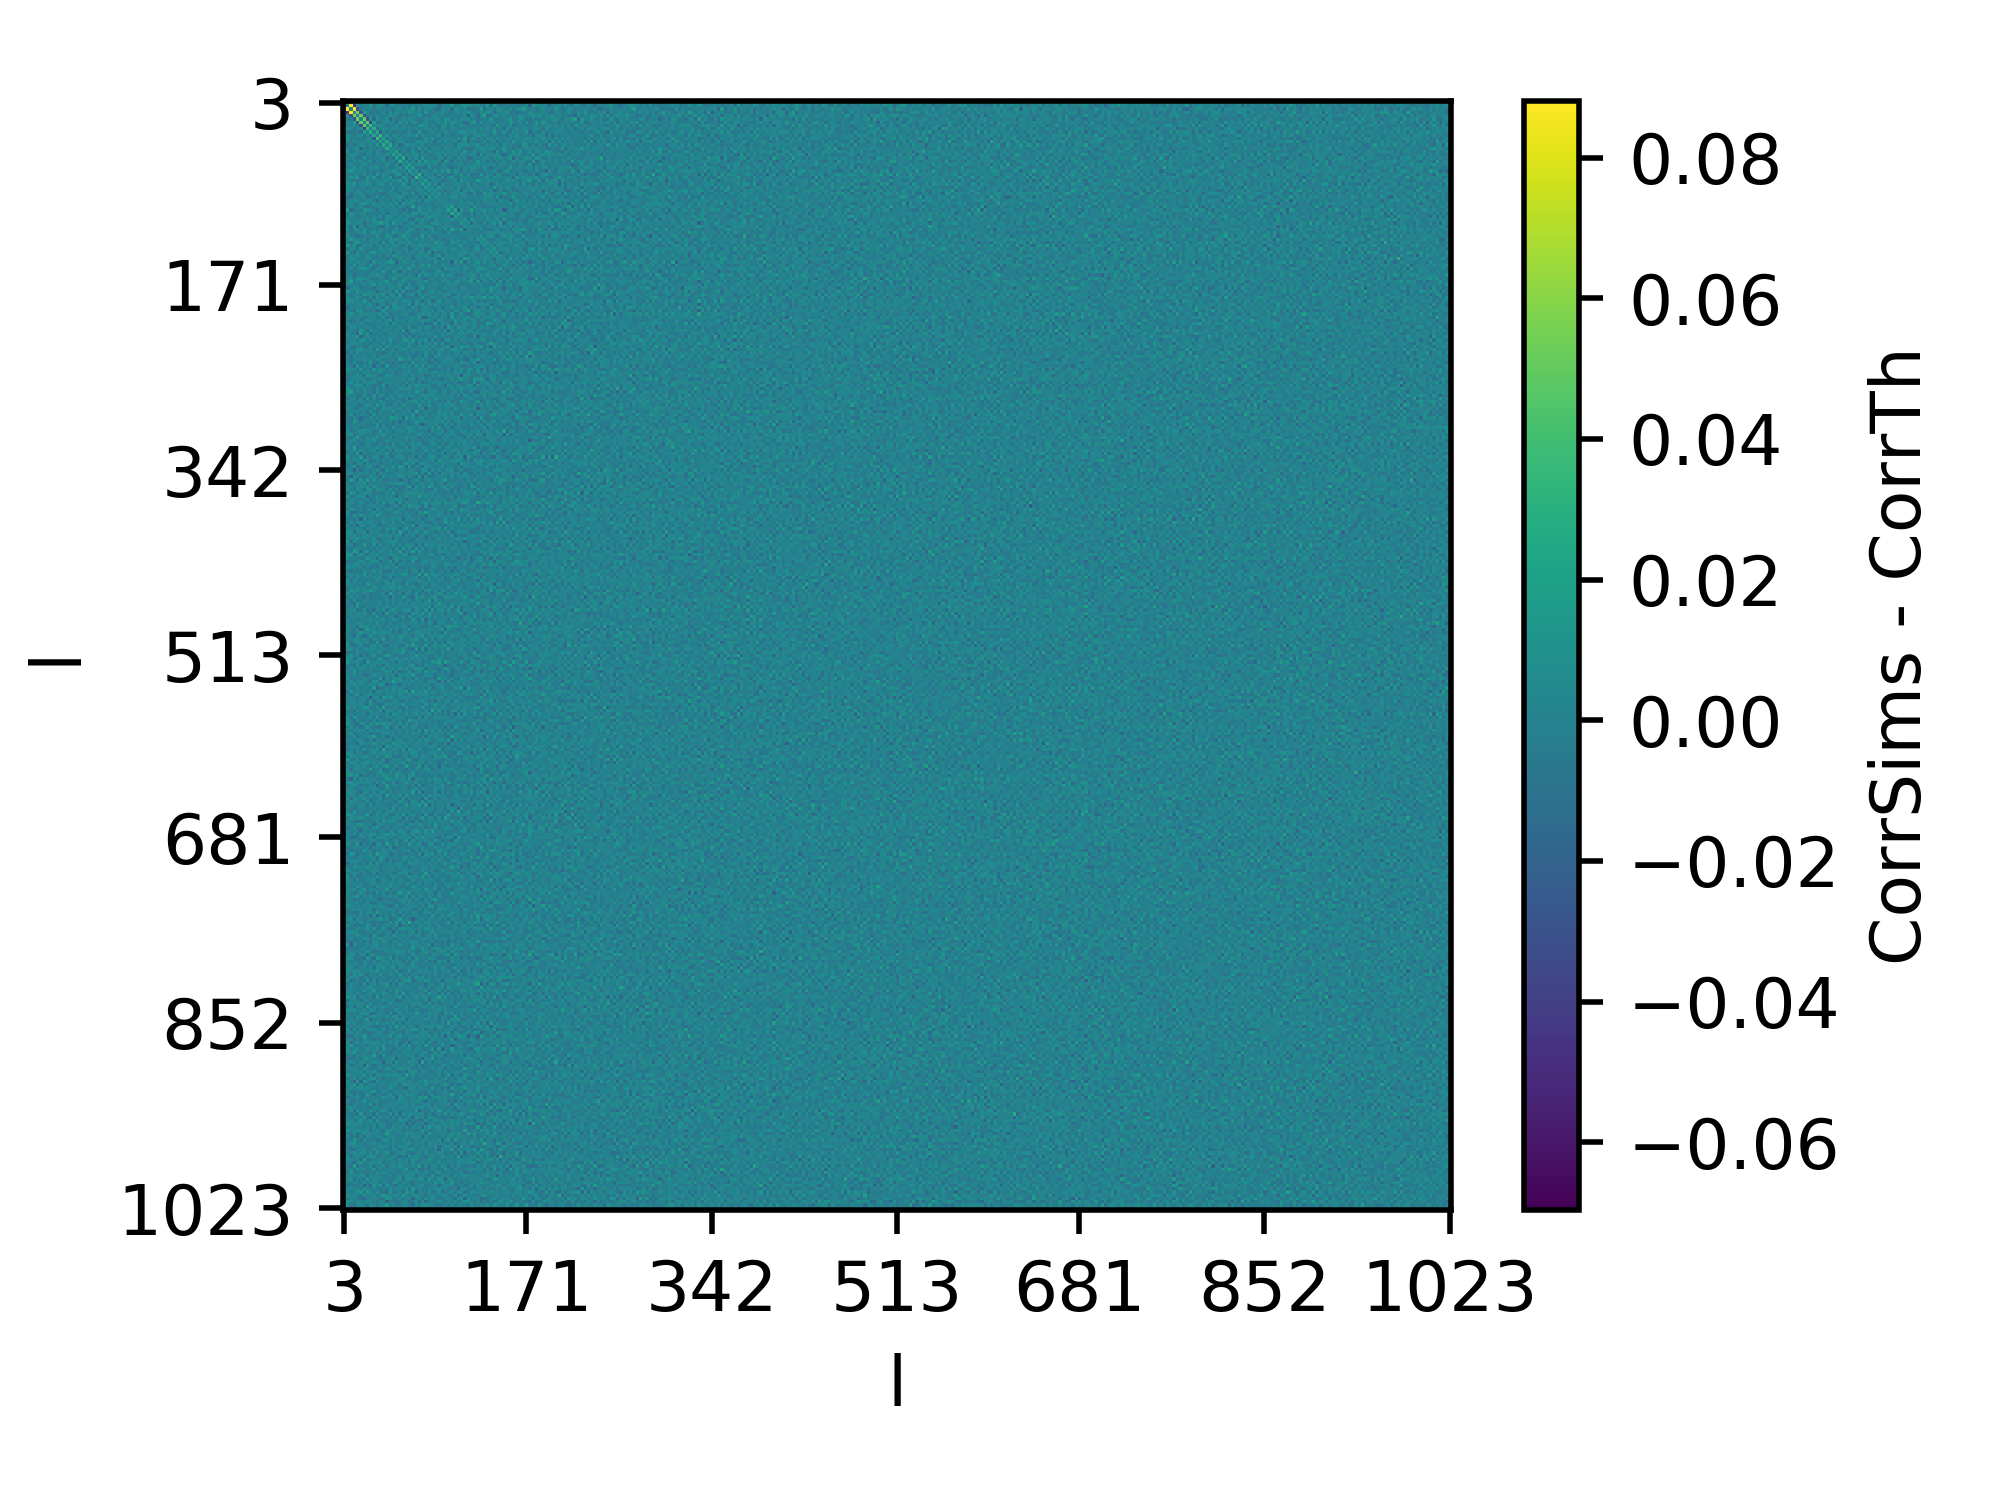
\includegraphics[width=\columnwidth]{./figures/run_sph_Efstathiou_EEEE_correlation_difference.png}
  \caption{Differences between the simulations and analytical approximation of
    the correlation matrices for the TTTT (left) and EEEE (right) cases.}
  \label{fig:TTTT_EEEE_corr}
\end{figure*}

These approximations do not work well for the B-modes, though. We can see in
Fig.~\ref{fig:BBBB} that we are not able to recover with accuracy the first
diagonal elements.


\begin{figure} %[htb]
  \centering
  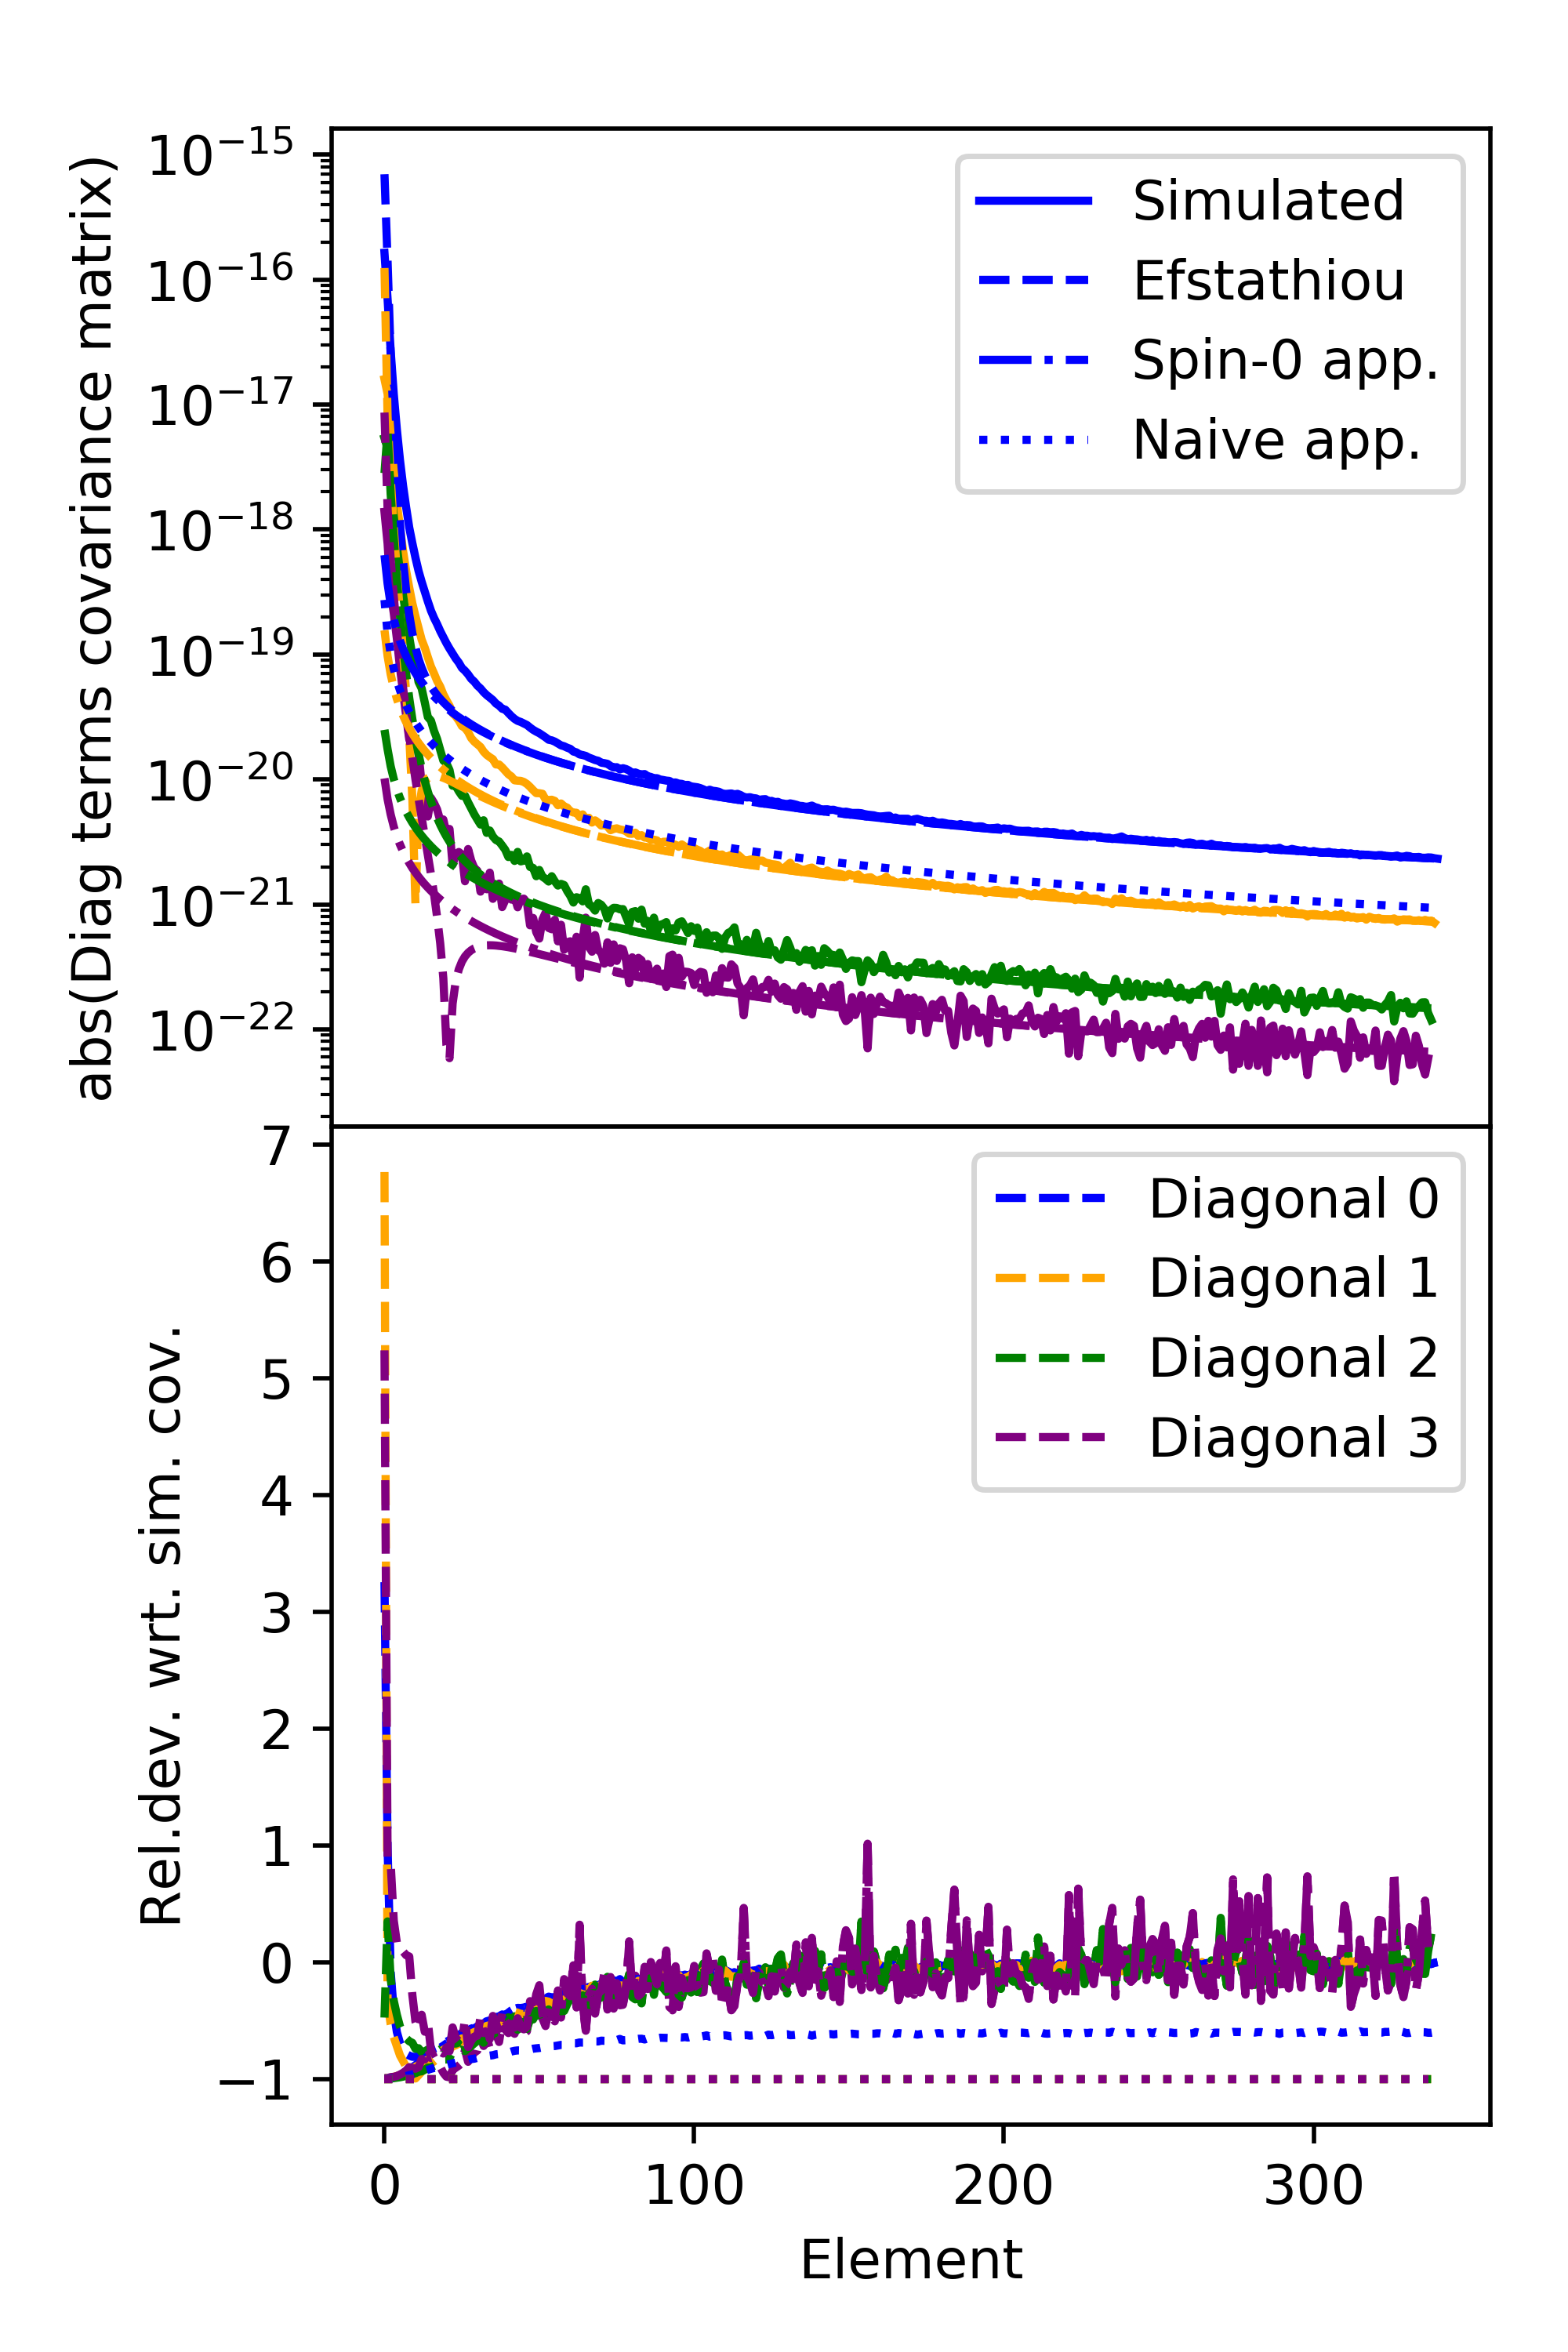
\includegraphics[width=\columnwidth]{./figures/run_sph_ALL_BBBB_check_diagonal_terms_4.png}
  \caption{The analytical approximation are not able to reproduce accurately
    the terms involving the B-modes. Here we show the most extreme case, the
    corresponding to the BBBB modes.}
  \label{fig:BBBB}
\end{figure}

Finally, the analytical covariance also works for 2-bin correlations. The
$\chi^2$ distribution for the covariance matrix of the modes TT, TE and EE
among two bins is shown in Fig.~\ref{fig:TTTEEE_chi2}. The eigenvalues
are recovered well except for the lower ones that diverge up to $20\%$ (see
Fig.~\ref{fig:TTTEEE_eigv}, this is not translated to any substantial
difference in the correlation matrices (see Fig.~\ref{fig:TTTEEE_corr}).

\begin{figure} %[htb]
  \centering
  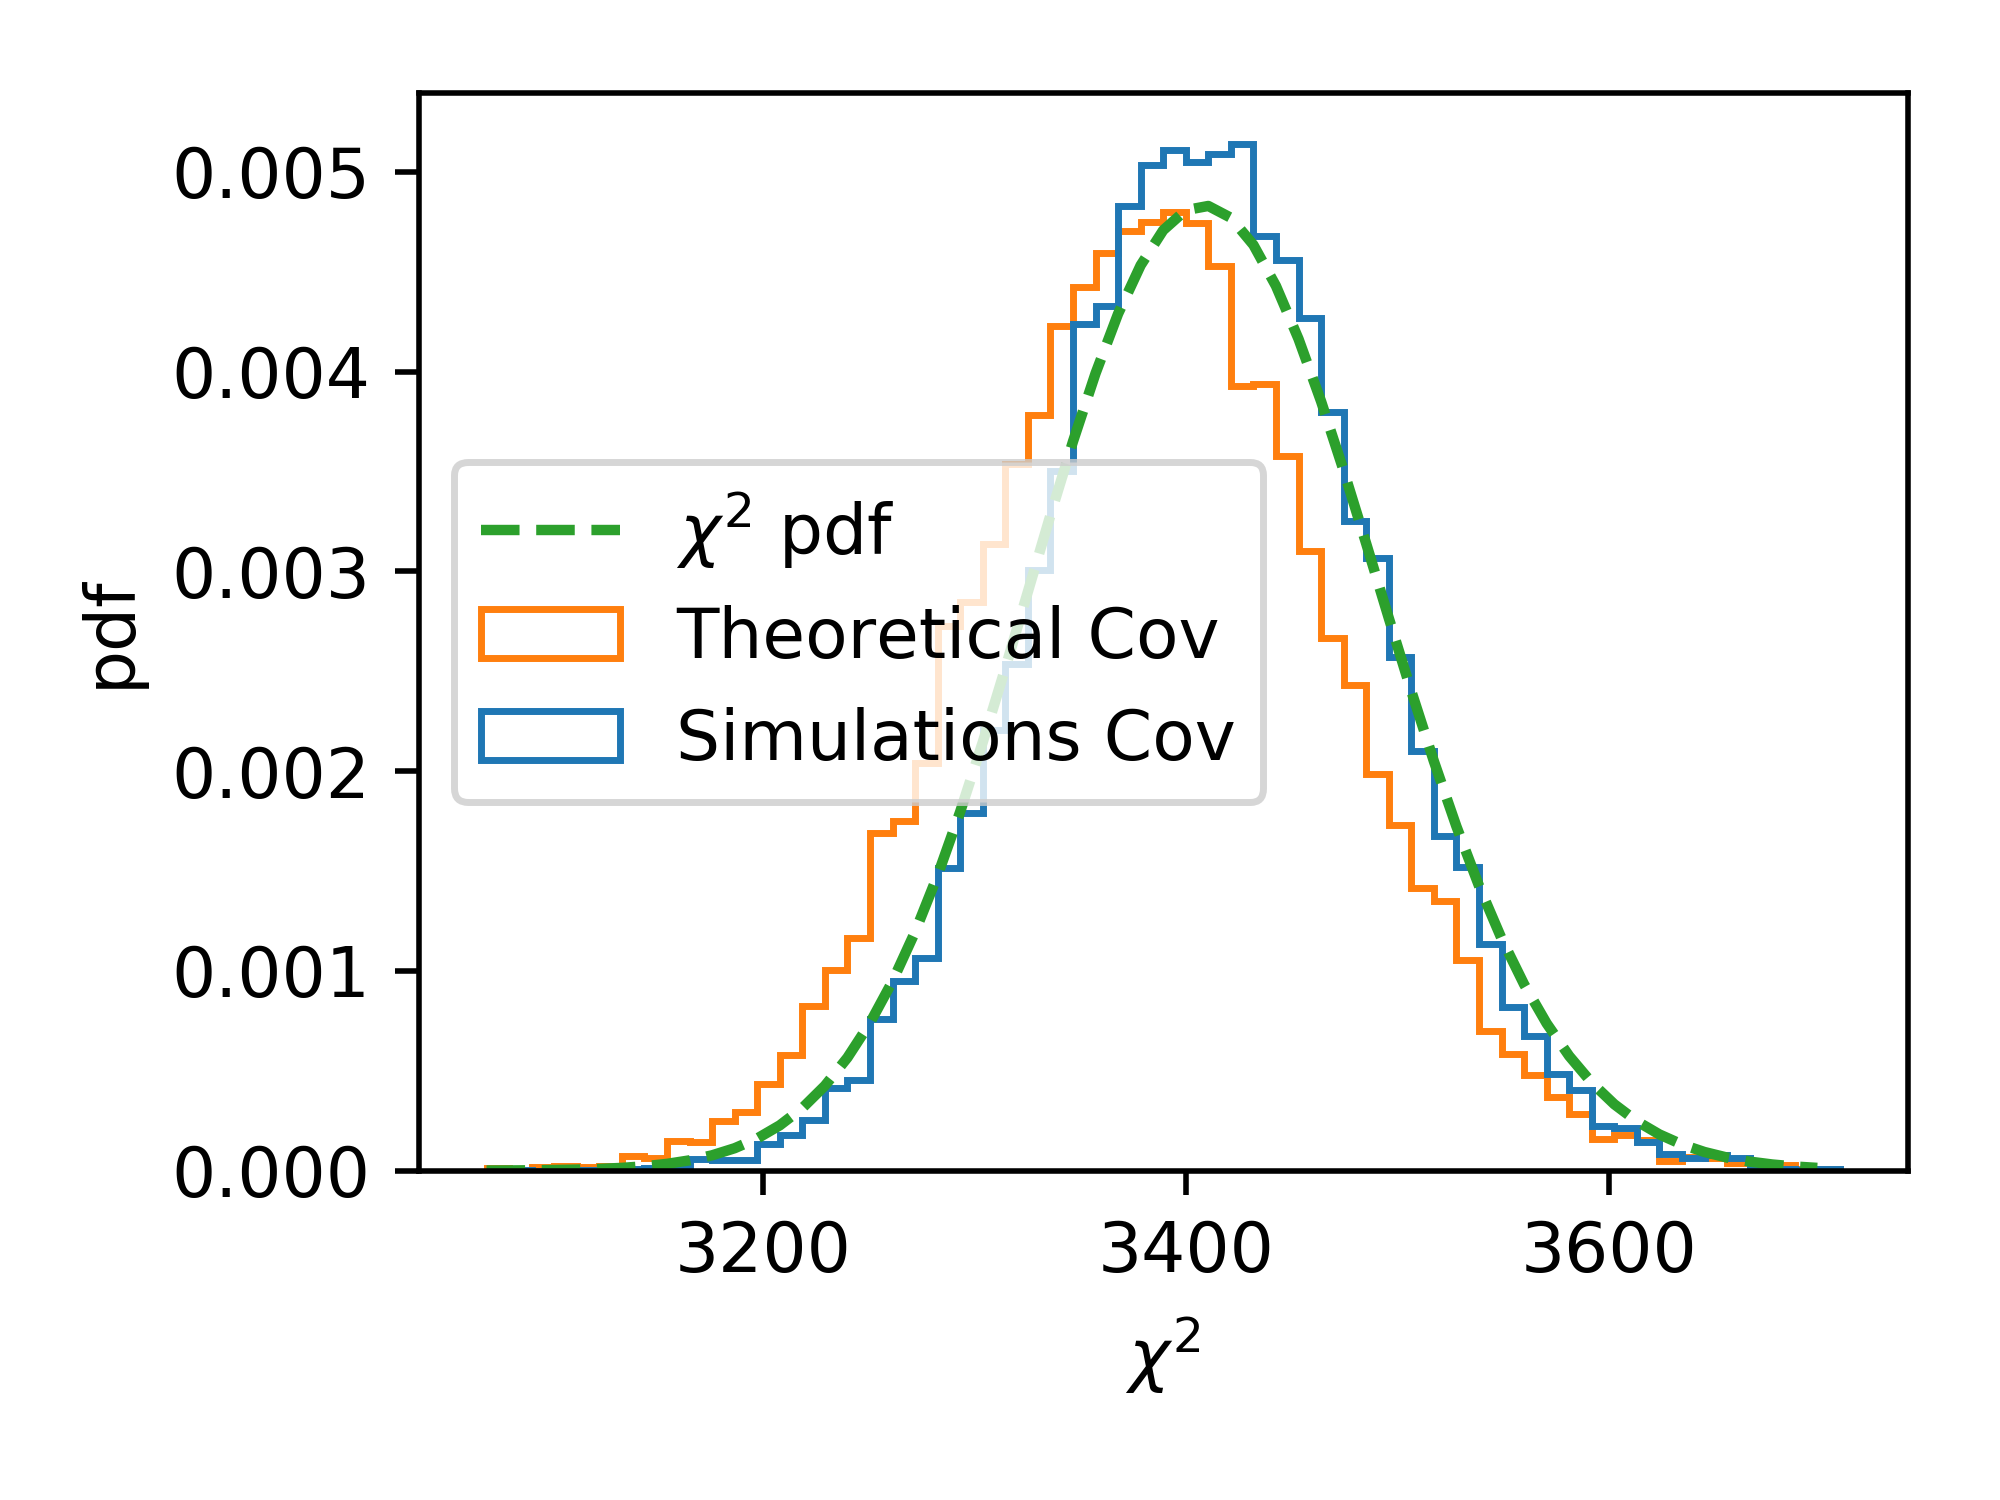
\includegraphics[width=\columnwidth]{./figures/run_sph_2b_same_mask_Efstathiou_TTTEEE_Full_chi2.png}
  \caption{$\chi^2$ distribution check for the full analytical covariance
    matrix for the modes TT, TE and EE among two bins.}
  \label{fig:TTTEEE_chi2}
\end{figure}

\begin{figure} %[htb]
  \centering
  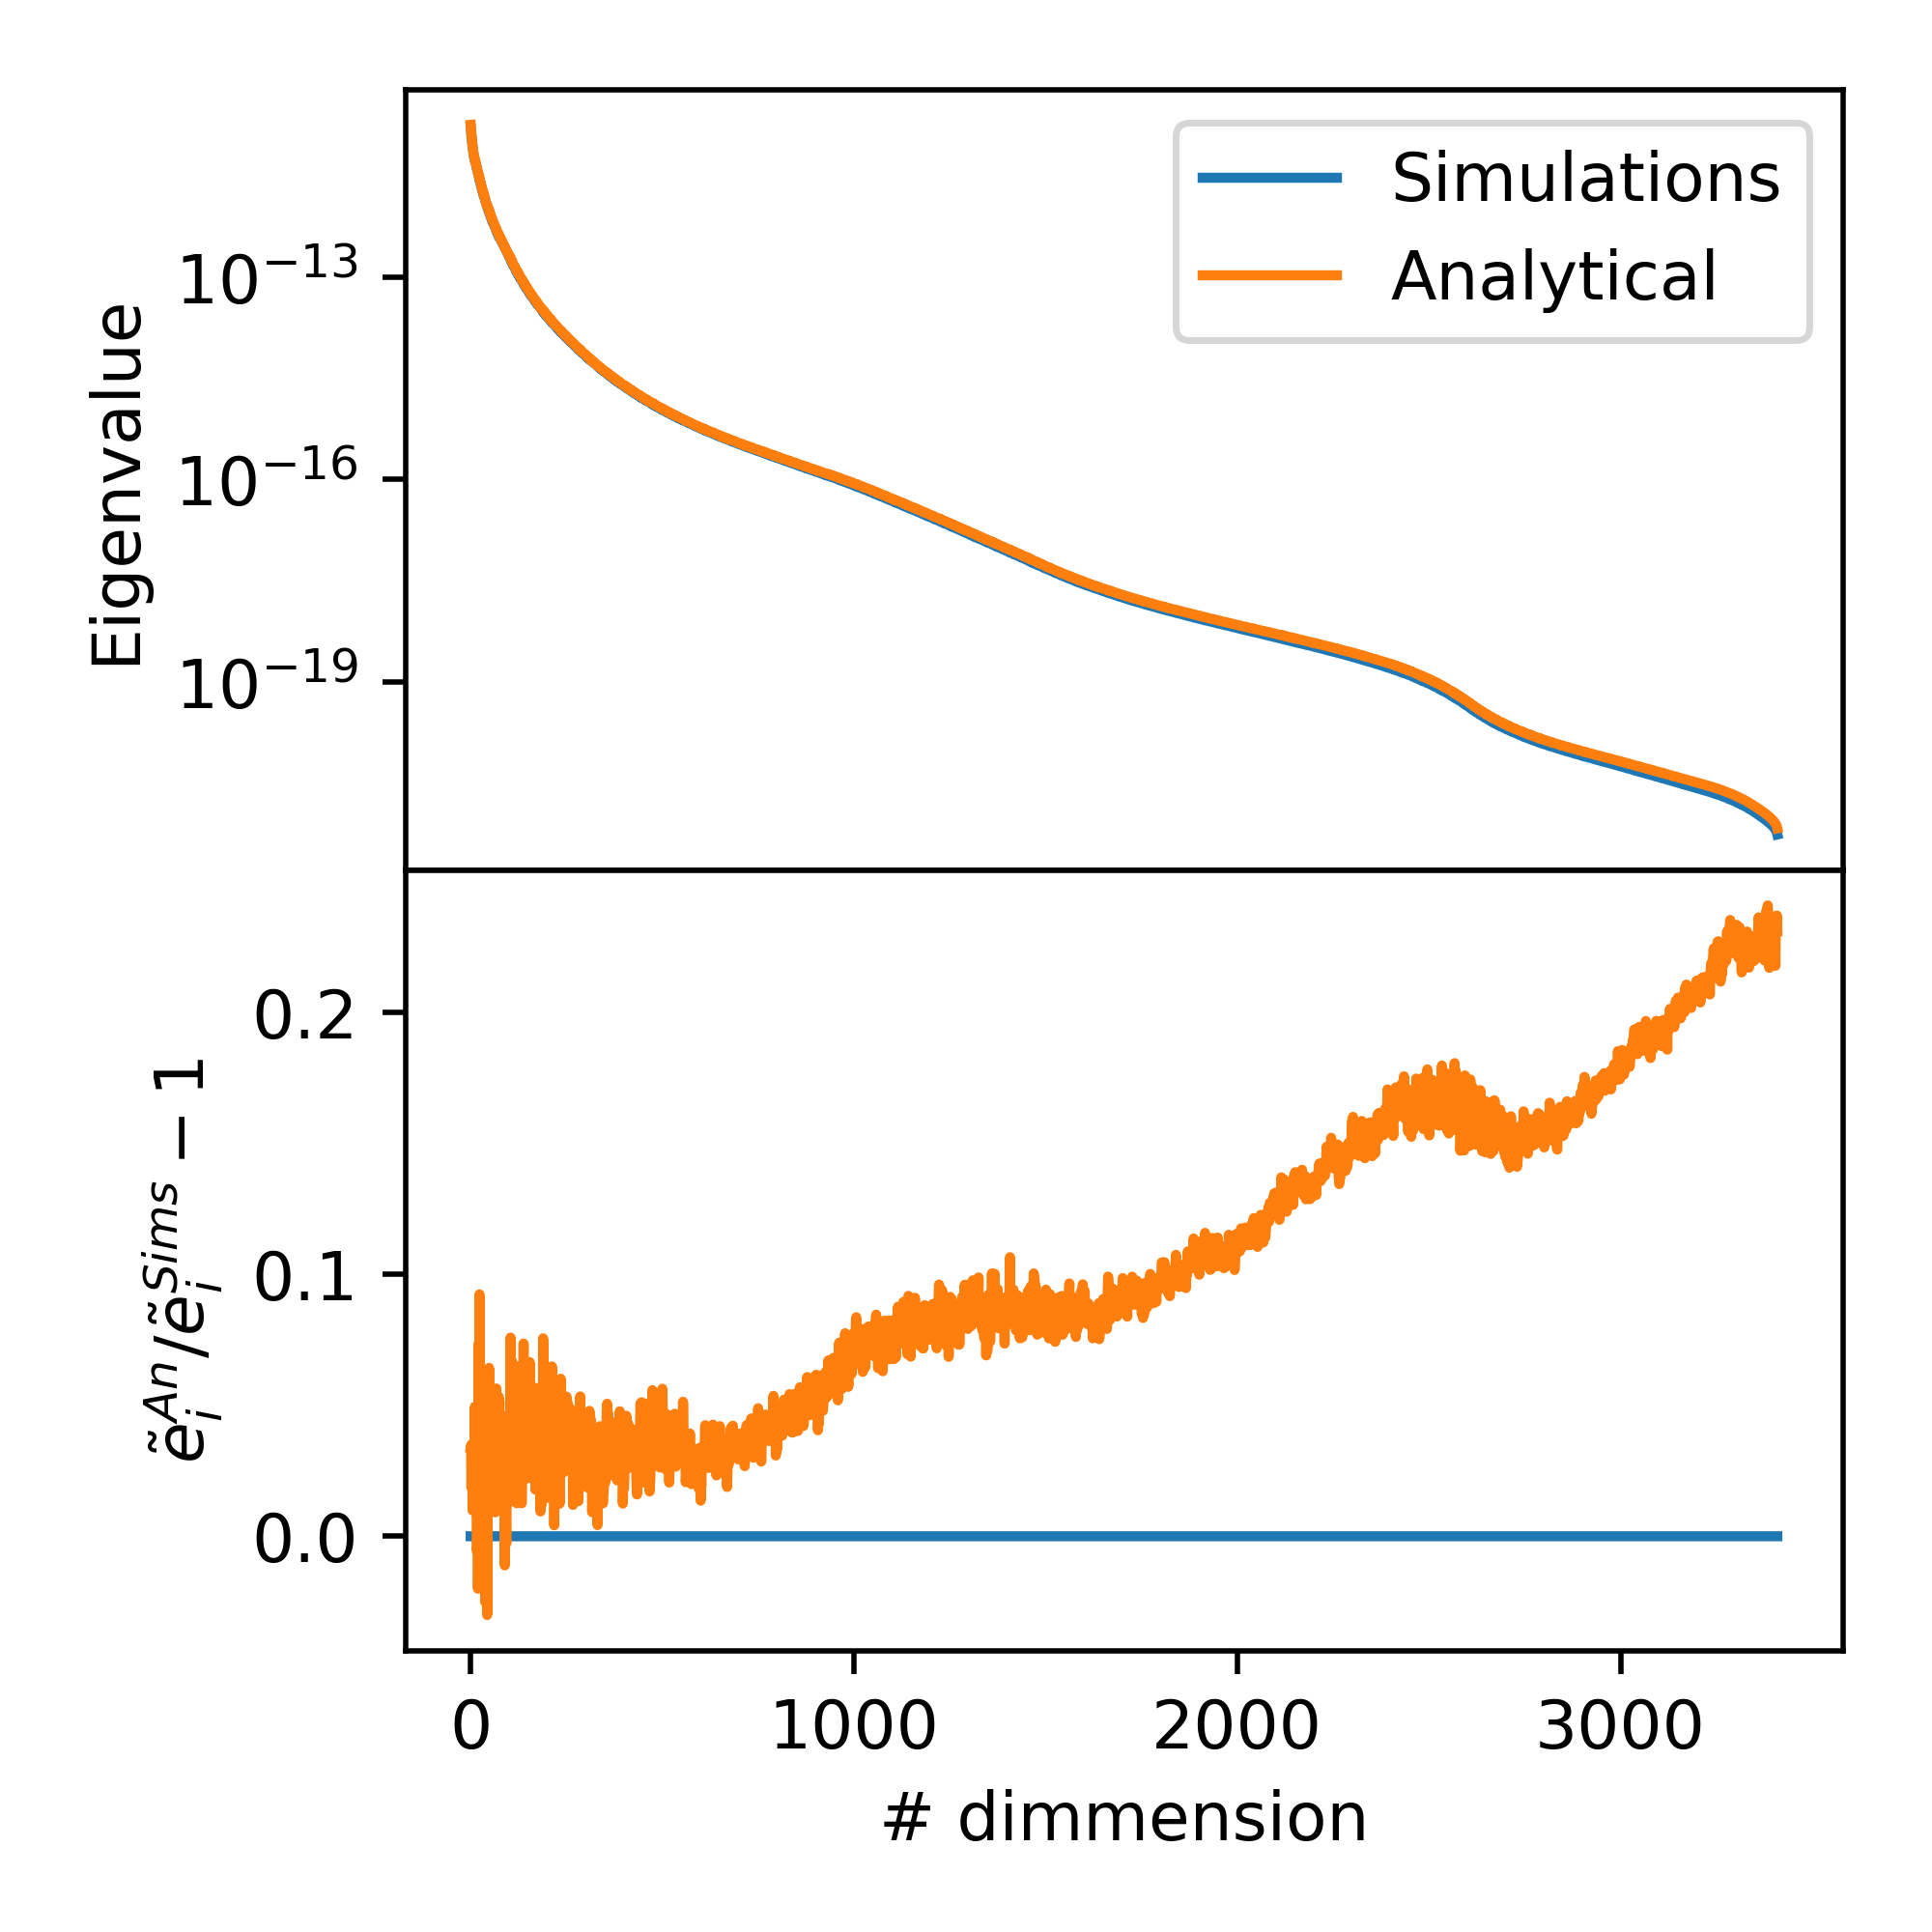
\includegraphics[width=\columnwidth]{./figures/run_sph_2b_same_mask_Efstathiou_TTTEEE_Full_reldev_eigval.png}
  \caption{Relative difference between the analytical and simulations
    covariance matrix eigenvalues for the modes TT, TE and EE among two bins.}
  \label{fig:TTTEEE_eigv}
\end{figure}

\begin{figure} %[htb]
  \centering
  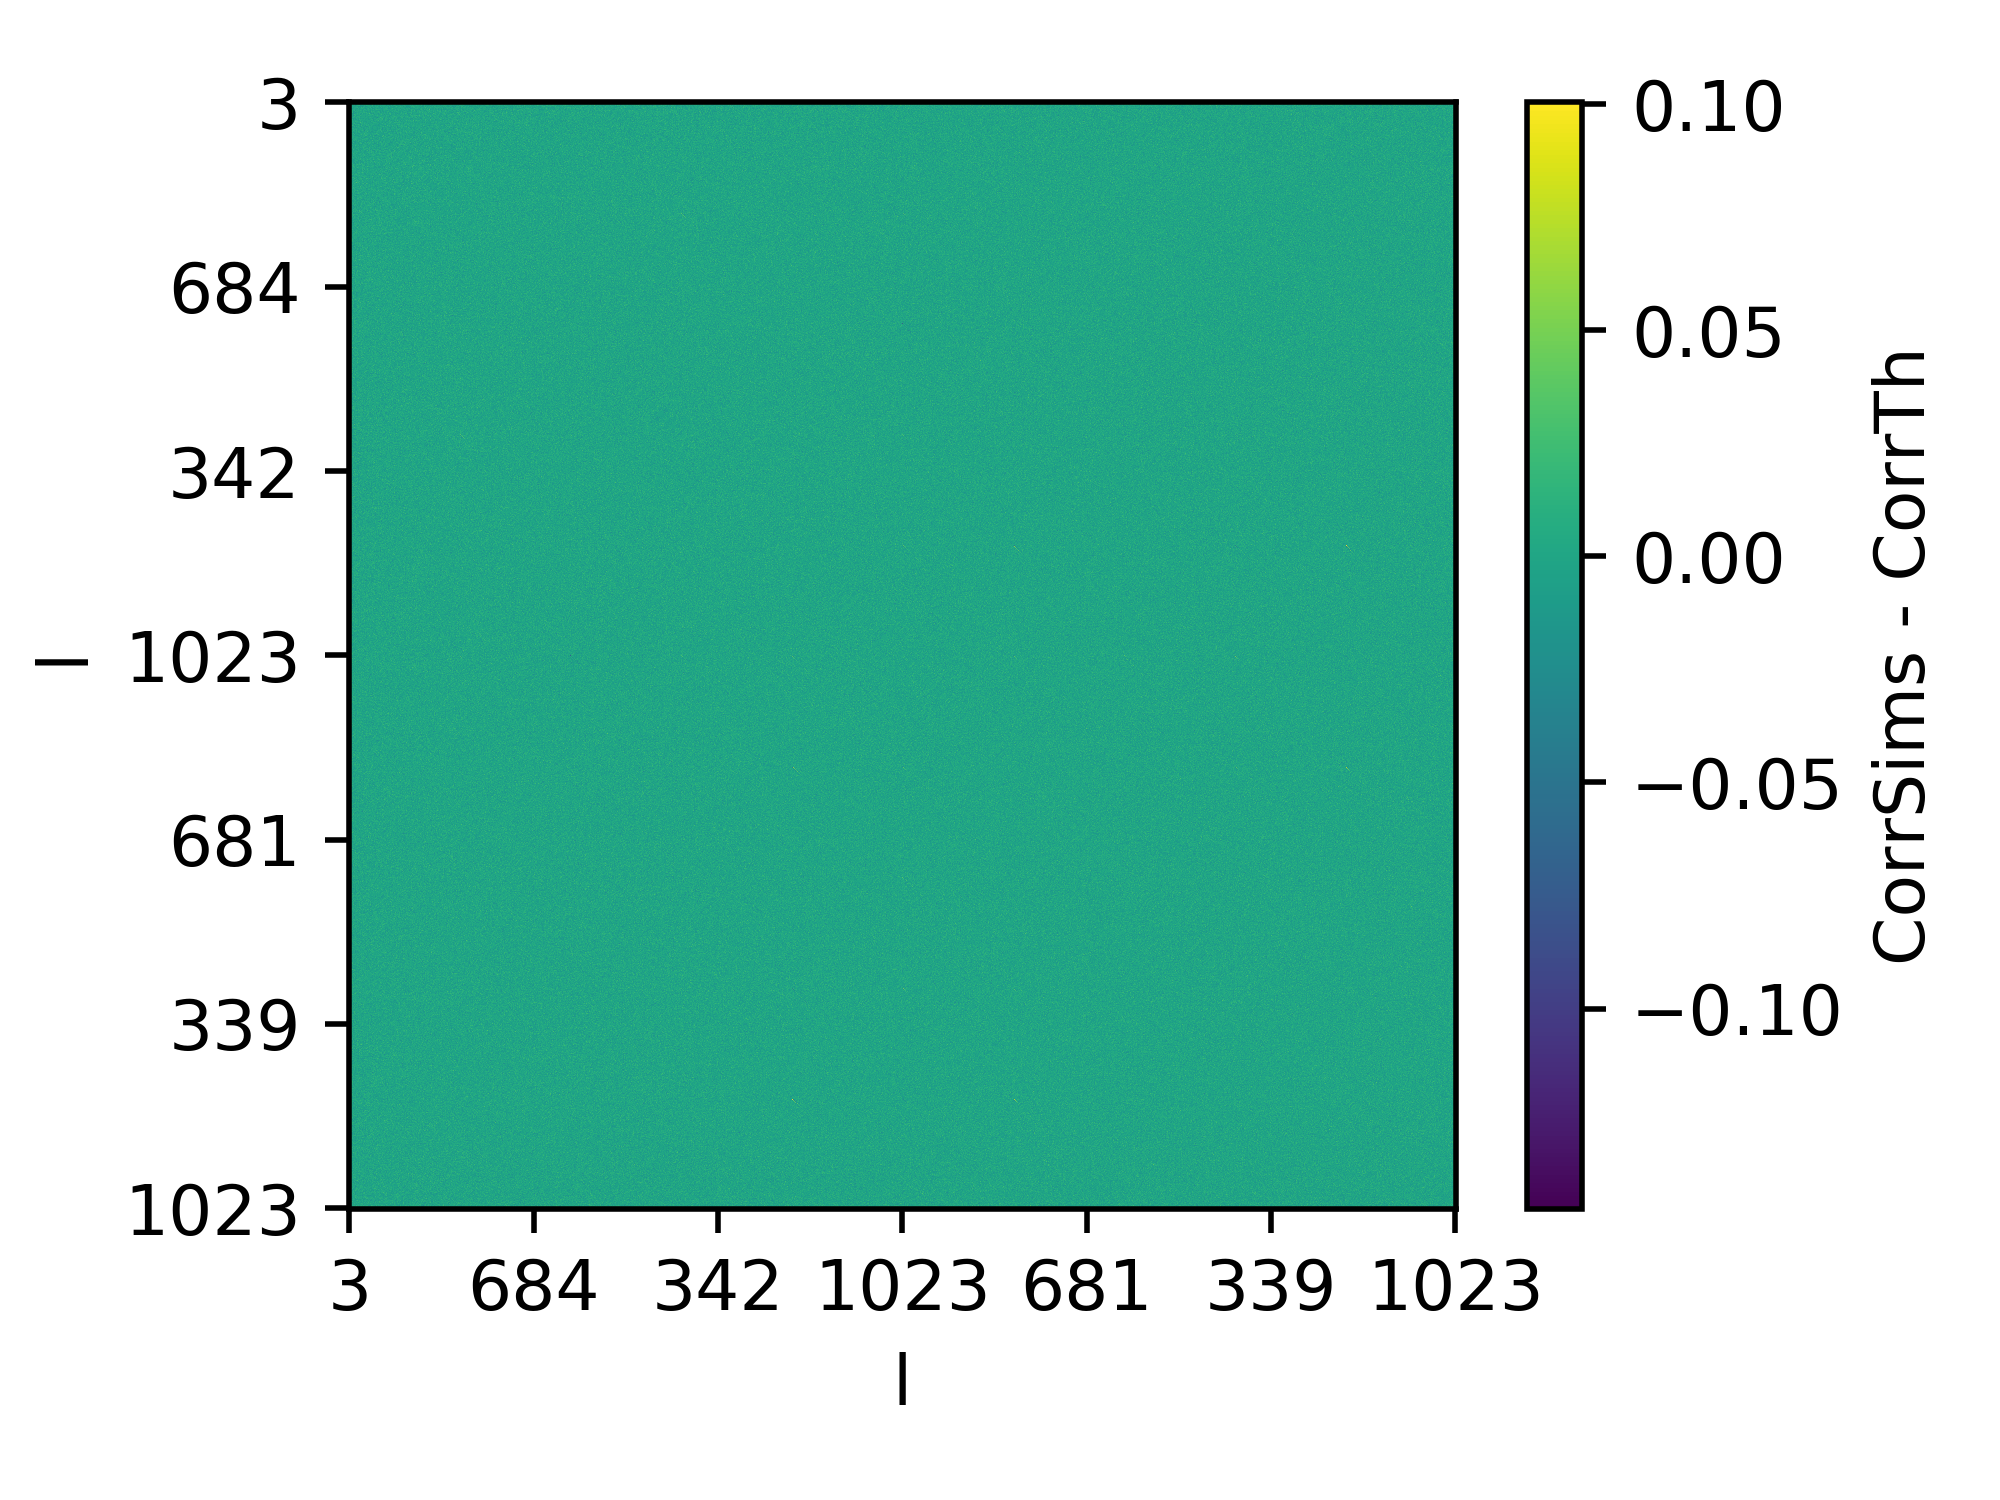
\includegraphics[width=\columnwidth]{./figures/run_sph_2b_same_mask_Efstathiou_TTTEEE_Full_correlation_difference.png}
  \caption{Difference of the correlation matrices of the simulated $\cl$ and
    the analytical one for the modes TT, TE and EE among two bins..}
  \label{fig:TTTEEE_corr}
\end{figure}



% The resulting power spectra was then used to generate a map of the sky and
% two random fields (one of spin-0 and other of spin-2), in turn. Their
% correlations give  are used to obtain the simulated power spectra. In order to
% find the real power spectra, it is necessary to subtract the contribution of
% the mask, which mixes the closest modes:
% \begin{equation}
%   C^{obs}_l = \sum_{l'} M_{ll'} C_{l'}\,
% \end{equation}
% where $M$ depends on the mask. In general, $M$ is not invertible and, in order
% to be able to recover the true power spectra, $C_l$, one needs to bin the
% $l$-space. The bin width is given by the characteristics of the window
% function and must be, approximately, of the size of the range of the mixed
% modes. That way, each $\tilde C_l$ is almost independent of the others
% $\tilde C_{l'}$, and $M$ is invertible.




\section{Discussion}\label{sec:discussion}

\appendix
\section{Flat sky}
\todo{Plot mascara}
\todo{Plot chi2 TT-TT TE-TE, EE-EE}

\acknowledgments

We would like to thank Eva-Maria Mueller for useful discussion. CGG is
supported the Spanish grant BES-2016-077038, partially funded by the ESF and by
AYA2015-67854-P from the Ministry of Industry, Science and Innovation of Spain
and the FEDER funds. He was partially supported by a Balzan Fellowship while
in Oxford. He would like to thank New College and the Department of Physics at
Oxford for their hospitality. DA acknowledges support from STFC through an
Ernest Rutherford Fellowship, grant reference ST/P004474/1.

\appendix


%\setlength{\bibhang}{2.0em}
%\setlength\labelwidth{0.0em}
\bibliography{paper}

\end{document}
